\documentclass{article}
\usepackage{blindtext}
\usepackage[utf8]{inputenc}
\usepackage[margin=1in]{geometry}
\usepackage{graphicx}
\usepackage{longtable}
\usepackage{tabularx}
\usepackage{float}
\usepackage{listings}
\usepackage[backend=bibtex,style=numeric,citestyle=numeric]{biblatex}
\linespread{2}
\graphicspath{ {images/} }
\addbibresource{DissertationPart2.bib}
\title{An Exploration into Building Three Clients for JominiEngine\\ Final Year Dissertation \\BSc Computer Systems}
\author{Rory Malcolm\\Heriot Watt School of Mathematical and Computer Sciences\\H00157560\\Supervisor: Hans-Wolfgang Loidl\\Second Reader: Chris Fensch}
\date{\today}
\begin{document}

	\maketitle
	\newpage
	\tableofcontents
	\newpage
	I, Rory Malcolm confirm that this work submitted for assessment is my own and is expressed
	in my own words. Any uses made within it of the works of other authors in any
	form (e.g., ideas, equations, figures, text, tables, programs) are properly acknowledged
	at any point of their use. A list of the references employed is included.
	
	Signed: \textit{Rory Malcolm}
	
	Date: \date{\today}
	\newpage
	\section{Introduction}
	\subsection{Aims}
	\subsubsection{Abstract}
	At Heriot Watt a historically accurate massively multiplayer online role playing game called “JominiEngine” has been created and improved over the years. The JominiEngine aims to provide a serious game for prospective students to learn about the time period it is set from gameplay. It implements a client-server model, the client communicates with the server using Google's Protobuf communication layer.\\

	This dissertation aims to produce a number of JominiEngine clients for different platforms; a text based command line client which runs on both Unix and Windows based systems, a graphical client for Linux desktop and a mobile client on the Android operating system. The implementation of these clients aims to expand the accessibility of the JominiEngine, currently the sole client available for the game is used mostly for testing purposes. After the client's development usability studies and technical studies will be carried completed, comparing and contrasting the user’s experiences with the features and complexities of each environment and how the development experience plays a role in the final product. The report will focus on the portability of the client server communication implementation and if the current client server environment lends itself well to the expansion of JominiEngine onto new platforms.
	\subsubsection{Aims}
	Through the development of the three clients for the JominiEngine this study aims to expand the accessibility of the game beyond the current implementation, which consists of a tightly coupled server and a demonstration client by giving users working, usable clients on multiple platforms. From the implementation of the mobile client more will be learnt about how the JominiEngine gameplay can be transposed onto mobile phones, within the constraints that come packaged with the platform, and what effect this transposition has on the overall user opinion of the product. The desktop and text clients will provide the study with a perception into what effect a robust user interface has on the user's experience of the product, comparing the simple text command line interface results from the usability study to that of the full graphic user interface will provide insight to this. This study will also aim to infer the technical capability of clients for the JominiEngine; Massively Multiplayer Online Role Playing Games by definition must be able to accomodate for a large number of connections at once; additionally these clients, especially the text client, will allow for the development of an automated testing suite to ensure that the server is capable at this level or performance. Technical metrics that are harvested from unit tests and telemetry performed while these are running will tell the technical side of the story with regards to their codebase's maintainability and extensibility, and with regards to their performance as the program is being executed, comparisons can be made between the clients and what effect they have on the system they are currently running on, these will be used to make informed criticisms of the final implementation of the clients with regards to code quality and scalability.
	\subsection{Objectives}
	\begin{itemize}
	\item Produce three clients
	\item All of the clients should implement the current JominiEngine protocol as standard.
	\item One of the clients is a text based client for internal and testing use.
	\item One of the clients has a graphical user interface and runs on a standard linux operating system (eg. Ubuntu).
	\item One of the clients runs on a mobile operating system which operates over mobile internet.
	\item Usability studies are conducted which show that the clients have been adapted to provide the best user experience for each platform’s constraints.
	\item The clients provide a scalable solution; multiple clients can run on a single computer with ease in order to test the constraints of the game server.
	\item As features are added to the server and protocol by other students working on JominiEngine the implementation of the clients should be flexible enough to easily incorporate any changes.
	\item The user should be able to move their account between devices and clients.
\end{itemize}
	\subsection{Evaluation}
	The success of the project will be evaluated by the delivery of three fully functional clients, the efficacy of these clients will then be measured, contrasted and compared with amongst other, through technical analysis. The evaluation stage is the mechanism through which consensus is established with regard to whether the project has been successful and if so, to what degree. Every objective can be considered, the experiences in implementing it, and what effect this had on the rest of the development process. The evaluation stage of this project will encompass a technical evaluation from which measurements about the performance of the clients will be extracted and compared and a user evaluation which will use a usability study to measure the opinion of users towards the clients, comparing and contrasting the scores between platforms.
	\newpage 
	\section{Background}
	\subsection{Literature Review}
	The purpose of the literature review is to explore the academic literature that surrounds the topics that the project will be covering, to understand where current research on the topics involved lies and what the best practises in each of these fields are.
	\subsubsection{Jomini Engine Introduction}
	The origin of Jomini Engine lies in David Bond's 2015 Masters thesis\cite{DavidBond} which outlines and implements a historically accurate massively multiplayer role playing game as an option for educational material. It aims to allow for students at a university to play a game that accurately reflects the period of study and from this experience learn more about the history of the period in which it is set, the role playing element of the game is designed to be as historically accurate as the medium allows for,  through the players gameplay they acclimatise themselves within the historical period in which it is set. JominiEngine is at its heart a turn based game, the user carries out actions which are then processed in the next turn, after the results of a turn have been displayed they then carry on with actions in the next turn. There are, however, some real time elements, such as the reporting of the success of a siege which is given to the player without a new turn occurring or the moving of a players army and character, these actions provide instant feedback to the player. Jomini Engine is split into three distinct areas of management, outlined in Appendix Item 4, these are the management of the player's army, the management of the fiefs that they own, and the management of family. The user controls a player which they move from fief to fief in a hex grid, the directions of travel possible are north east, north west, east, west, south east and south west, as they travel from fief to fief the armies which they have ownership over travel with them. There is then army management, this allows for the user to hire more troops using funds they have acquired in order to have a higher chance of successfully sieging other fiefs. The user then has a degree of control over lineage via the family management mechanisms; the functions of succession in the event of a player death, if the user suffers a character death because of a failed siege gameplay can be continued through a reared successor. Finally, there is fief management, this allows for the user to set the levels of investment they have in the the fief and the rate of taxation, the user can hire troops who are without an army from the fiefs they own, therefore it is important for a user to gain control over new fiefs as they provide a route with which to expand their armies. All of these individual functions are then combined by the sever, who on each game step computes the results of the actions the player has taken and updates the game state accordingly. JominiEngine aims to be massively multiplayer, with players connecting from distributed clients on different networks to a singular server which they send and receive information from, this allows for the players to play from multiple locations without losing their progress as long as the player is connecting and playing on the same server every time. The current status of development takes the form of a test script, this runs the server and the client as part of the same codebase, with tight couplnig between the operations of the server and the client. The test script is executed a number of operations are performed on behalf of the player, the output is presented to a command line interface as each operation is completed. This application has no mechanism for user input an only exists as a showcase to show that the functions of the underlying server work. The expansion of the client base aims to provide three direct options to a user for gameplay, offering them choice depending on what the context they are playing within demands.
	\subsubsection{Game Design Decisions}
	As gaming moves beyond being a special interest hobby and into the mainstream the popularity of MMORPG’s has swelled; for example Blizzard Inc, the creator of the 2004 released \textit{World Of Warcraft} reported in 2015, 11 years after the games release, that they had a player population of 5.6 million active users. Efforts to explore the popularity of MMORPGs have been carried out\cite{Christou:2012:EPP:2367616.2367630}, studies show that the usability of the game has a positive effect on engaging players but the popularity of the MMORPG genre cannot be inferred from this, only that well-made, usable games are attractive to players. There have been other attempts to analyse the community aspects of MMORPG’s effect on the player base\cite{DoThoseWhoPlay}, research has concluded that while players initially struggle to immerse themselves fully in the world after some effort is spent they find themselves inside of complex social systems which mimic and alter real life, some respondents reported that the social aspect was the most important part of their gaming experience. This aspect of gaming can only be found in multiplayer games where interaction with other players is possible. The study reflects on the fact that the World of Warcraft players it surveyed do not see a point in playing alone, the social aspect of the game is so great that they do not see their gaming experience as complete without it. This is explored further when looking at the\cite{Hainey:2011:DMO:2304793.2305216} difference between the way multiplayer gamers and single player gamers in higher education view their experiences, they noted that online gamers see competition, challenge and recognition to be much more important than offline gamers and that online gamers believed gaming to be “more of a social activity, less of a waste of time, more interesting, more worthwhile, more enjoyable, more valuable, more exciting and less of a lonely activity”. This yet again confirms the perception that online gaming and offline gaming, while in the same field of interest have separate mechanics and are different experiences gameplay wise and socially. Then, looking at the personalisation aspect of MMORPG’s and how that effects the user’s perception of their gaming experience; players feel RPGs place them in the context of the situations the game is providing and do not feel the character is a separate entity\cite{bowman:2012:EPP:2367616.2367630} this further strengthens the “MMORPGs are inherently social and personalised via a product of game mechanics" hypothesis. JominiEngine aims to become a serious game, that is, a game which has a central learning objective as opposed to a gameplay one, the players are driven to achieve this learning objective by the mechanisms within the game, the intended result is that players are to learn through playing. While normal games aim to pass the time, providing the player with entertainment, serious games aim to provide the player with a learning experience, a new method of studying. JominiEngine's historical accuracy aims to help a student of history familiarise themselves with the time period it is set and by playing they learn more about the context and actors at play during this period. This has been explored academically in the past\cite{seriousgames} and history especially has an avenue for study via serious games due to the fact they can immerse the user fully into the time and world of study.
	\subsubsection{Game Interface Decisions}
	The project shall consist of the implementation of three clients, a text-based command line client which will be lightweight and portable with the potential to run on multiple operating systems, a graphical user interface for easier usage by newer users which can run on more powerful machines, and an Android client for use on mobile phones or tablets for playing in a mobile context. When considering the implementation decisions for an MMORPG client it is important to understand how the user will be interfacing with the game and what options are best for the platform the user will be running the game on, taking into account the limitations and constraints of that platform. Most of the work surrounding mobile gaming interfaces explores the new experiences that can had due to the player have access to new sensors such as a accelerometer or the phone's GPRS service. However if the mobile client is considered, questions must be asked with regards to what limitations are placed upon it via the hardware. Phones have smaller screens than desktop computers so there may need to be some modification of the user interface in order to account for this. As mentioned before, usability is a main driving factor in user attachment to games\cite{Christou:2012:EPP:2367616.2367630}, it is not enough for the client to offer a command line version for mobile and still have users come away from it as immersed; these interfaces are designed for machines which have hardware keyboards as their main method of communication. The mobile client's interface must be designed from the ground up for the platform, taking into account for example, the large touch screen most smartphones have. The user could navigate fiefs by dragging their fingers around a map similar to the current hexmap used in the test client implemented in Helen Rankin's masters thesis\cite{helenrankin}, this would provide a mobile-first user interface using techniques more natural to frequent users of the platform. The text client will use a Read, Evaluate, Print, Loop style interface that is common in command line applications such as Python's IDLE\cite{python}, the user is prompted input information by the program, the user then inputs the step they wish to take, the program evaluates their input, prints the output and the process is repeated again. Using such a common interface for command line tools alongside a help menu should make for a better and more familiar user experience.
	\subsubsection{Mobile Game Development}
	When considering development on a mobile platform their must first be considerations with regards to the mobile operating system that the app is being developed for; there are a lot of options available on the market but the two main players in the industry are iOS and Android. If iOS is considered, some problems arise that could hinder the development process, first of all to get access to the full suite of development tooling there is a subscription fee to publish apps and the XCode IDE which is used to develop  apps for iOS only runs on the Mac platform. There is tooling which aims to open up the development experience for iOS such as Microsoft's Xamarin\cite{Xamarin} which allows for a developer to write C\# code which cross compiles for running on both Android and iOS but this still requires a development license and an accessbile Mac machine for compiling the code to an executable which can run on an iPhone. Android on the other hand is fully open source and can be developed for on any platform, natively it runs Java code but there are a large number of languages which have been ported to the platform for running on its ART virtual machine such as Scala or Jython - an implementation of the Python programming language which compiles to Android RunTime bytecode.
	\subsubsection{Mobile Networking and its Effect on the Gaming Experience}
	There has been some research into the effects of mobile network’s temperamentally on a players gaming experience. One research paper\cite{6098224} looked at the frequency of disconnections on a wireless ad-hoc Quake3 server and found that the quality of connection meant that “the number of disconnections due to packet losses were so frequent that very few parties ended with all participating players “. Network stress’s effects on the MMORPG gaming experience has also been explored; Everquest2 was used as a testbed to monitor the effects of latency on a players “skill”, defined as the time it took for the time it took for players to complete tests in the game\cite{Fritsch:2005:ELN:1103599.1103623}. They found that at 1250ms of ping it became unplayable, however it is important to note that the context of this test was in a real time game and not a turn based game like JominiEngine which should mitigate the effects of latency due to real-time user input and reaction’s importance being diminished. There has been some attempts to look at solutions to mitigate the effect of mobile internet technology on the gaming experience\cite{Wang:2012:CMG:2331675.2331679}, suggests that there may be an alternative to the traditional client-server model utilised in JominiEngine which would better facilitate gameplay over mobile networks. They suggest a model which incorporates a game engine server which is used to compute and render the frames based on the actions the user takes and then these are relayed back using a streaming server similar to how video traffic is transmitted over the internet. To implement this in the context of the JominiEngine would be an arduous task outside of the scope of the project and they conclude that their research is experimental and would only be successful in certain contexts.
	\subsubsection{C\# or Java}
	When comparing C\# and Java it is important to note that the languages are very similar and are inspired by each other, there is no great limitation to picking either choice. However, there are advanced language features and tooling that exist for one platform that the other platform does not have access to, this drives the decision making process. C\# for example provides a language feature which allows for the developer to construct variables with an anonymous type, no alternative exists in the Java ecosystem, anonymous types are useful when the developer needs a quick way to encapsulate data inside an object while reducing the bloat that is found in systems that have too many classes and components. They are especially useful when dealing with data which does not have a concrete type like when accessing information from JSON input, or in foreach loops where the developer wishes to infer the type of the object that is currently being accessed in the list from the type of the object the list is a collection of. Java has no implementation of anonymous types, but there are also other features of C\# for which Java does not have a analogous implementation. The .NET framework has a tool called LINQ which is used to perform structured queries similar to the sort seen in database languages like SQL on relational data stored in memory. This is an incredibly powerful tool at the developers disposal in certain situations when there is a need to pick certain information from a large dataset or when they wish to iterate through every item in a list and perform an action if a certain condition is met. Java has similar attempts to replicate this mechanic but they come from external libraries which are provided by the community and are lacking documentation and native support. The applications of constructs like these in an MMORPG client are clear, information taken in over a network needs to be stored and analysed before operations can be performed on it and anonymous types provide a solution to that, LINQ provides data manipulation utilities which could be used to lookup information about items the user may wish to find. For modern game development the Unity library is one of the most popular, with a massive amount of industrial backing and a large community as well as being free for personal use\cite{Unity3D}. The Java community has had attempts at creating similar engines, for example the JMonkeyEngine\cite{JMonkey} but they do not have the support or features of Unity, such as their fully fleshed out Android development kit. For the development of the initial text client, which will be used to ensure that the protocol implementation is correct before it is ported to Unity and Android, both C\# and Java offer tooling for creating powerful console based applications. Libraries that make the console development easier take the form of the JCurses library\cite{JCurses} for Java, and the native .NET console libraries for C\# offers a robust set of tools for the platform as well. A large amount of modern game development is carried out in C++, and there is a lot of incentive to follow this choice, it offers a robust, close to the hardware platform to develop games with. One of the examples of library support for C++ that make game development easier is the Vulkan graphics library\cite{vulkan}, this is a new, state-of-the-art low level graphics library, it allows for programmers to get as close to the hardware as possbile when they need to write the graphics component of their game engine. Vulkan is not aimed for end users to develop their games with but is meant to allow building blocks for tool developers to build off in order to give game developers more power and control of their system, the problem with this amount of power and low level access is that it is too complex to develop a suitable working user interface for the desktop client in the time allotted. The bare metal performance essentialist development experience is mostly important in the context of the server, it will be facilitating a large number of connections at once and needs to be written efficiently to give the largest amount of users a quality gaming experience as possible. Due to the fact JominiEngine is a turn based game there is no real time graphics component, there is no need to constantly render the scene hundreds of times a second as there is in for example first person shooters, this means some liberty is afforded when making the choice of language. C\# offers some extra advanced language features like LINQ that has been described earlier in this section which make develpoment easier but if needed it can perform low level actions via the unsafe keyword\cite{unsafe}. When code is in an unsafe section in C\# it allows for the manipulation of memory at a very low level, similar to C++'s memory management capabilities, through the unsafe keyword the programmer has the best of both worlds available to them and this plays a role when considering the choice of language for the project.
    \subsubsection{Modularity}
    Since this project encompasses three clients which all implement the same protocol there will be a degree of similarity in the codebases of all three clients, especially on the communications layer. Moreso between the text client and the desktop client, they will be written in the same language (C\#) and may use the exact same classes and methods to communicate via Protobuf\cite{Protobuf}. Protobuf allows for the quick serialisation of data to a standardised, shared format between the client and server and is particularly useful when sending information in real time as occurs during multiplayer gaming. The main issue with regards to the portability of the project are the user interface components, the user interface for each client must be designed from the ground up, sometimes piggybacked off a previous communications implementation and in the case of the mobile client off a completely new communications layer. The user interface for the text based client will be written in C\# using the inbuilt console manipulation libraries it has\cite{ConsoleClass}, the desktop client with Unity\cite{Unity3D} and the Android client will use Android's built in user interface libraries\cite{AndroidUI}. Current clients for JominiEngine such as the one in Helen Rankin's masters thesis\cite{helenrankin} implement a user interface in part using the HexMapGraphs utilty of the QuickGraph library\cite{QuickGraph}, this implementation is rather simple however and does not allow for the flexibility of features that will be required for a high quality client, therefore there is no option to port or take inspiration from an older client on the user interface side of development. Portability also encompasses the ability for extending the code base in future, if a client aims to be portable and is designed to fit this specification it should lend itself well to this. An example of this could be the religion feature currently being developed by another student, if this is implemented in time for the usability study of the client should be designed in a way in which the work that needs done is accommodating for that feature inside the protocol and adding the user interface mechanics to handle it, the codebase should be decoupled to make extension by another developer in the future as easy as possible. 
    
Due to the client server relationship the majority of scalability work comes from the server, which must be designed in a way and hosted on a fast enough machine to facilitate multiple clients connected and sending requests to it at once. The client could help with the scalability requirements of the server by implementing some techniques which lower the amount of requests that are needed for the user to play the game. One of the techniques that could be implemented could be some form of caching system, or a move to a different model such as a peer to peer system. There has been some exploration of the latter academically\cite{1354485} suggests that a move away from the client server model would require a significant amount of work, if players are not evenly scaled across the regions of a server it could cause latency issues which would lessen the players quality of experience. Player authentication is also a problem in this model, players have no central server to report to and validate that they are who they say they are, peers in a peer to peer model would need to be trusting of each other or implement a solution to mitigate this. It would require siginifcant reworking of the protocol and server of JominiEngine to implement such a model and the returns would not be as bountiful with the small number of players that JominiEngine is used by or tested with at this stage. Caching as a solution to reduce the amount of traffic going from the client to the server could be useful, there are libraries for both C\# and Java which provide a solution for this, CacheManager\cite{CacheManager} for C\# and Caffeine\cite{Caffeine} for Java. These could be used to consistently store the fiefs that currently surround the user so that information about them can be retrieved without having to carry out the full protocol request, not only would this save server resources but it would also be faster on the client side due to the information being stored in RAM and retrieved from there faster than a full web request. From a client perspective "scalability" means acting efficiently when communication with the server, and scalability during testing would mean that multiple clients can be run at once on the same machine or on the same host environment inside of virtual machines without them being too process intensive to do so. Due to the fact the text client uses limited user interface resources it is a sound choice to ensure that the implementation of the underlying protocol is correct, with the mobile and desktop clients being evaluated in the usability studies to ensure they work correctly. These individual components that form the build in order to improve portability and stability are helpful with regards to the modularity of the client, all parts of the client are decoupled from each other to the maximum extent that is possible, the user interface component is isolated from the networking component and the networking component from the event handler. Modularity aids with scalability, if a section of the codebase is blocking progession or is not fit to handle the level of traffic it needs to be replaced. Replacement of a component in a modular codebase is much easier than in one which has tight coupling, an example of this in the context of JominiEngine could be the networking layer, if this was found to be inneficient replacement would be easier, the other sections of the program are not exposed to the module through anything but method calls, as long as the API remains the same nothing else must change. This modularity lends itself to further expansion of the JominiEngine client ecosystem; if independent components exist they can be taken from one client and used within another, this speeds up the development process and keeps clients more maintainable, if an error exists within the networking codebase, for example, it can be fixed in one location and applied to all others.
	\subsubsection{Usability Surveying}
	The usability survey is the key component of the user evaluation, it is from the results and trends of this that the score for the social side of the system can be derived. There are a number of pre-written usability assesments which have been proven to measure the opinion of the subjects, one of these is John Brooke's SUS form\cite{Brooke96sus:a}(Appendix Item 3). This provides a framework to score the users perception of any given system and is used often in industry and academia, it uses a lickett scale to grade how much a user agrees or disagrees with a statement and from the collection of scores they give a picture of their perception can be built. The individual user grades can then be taken and viewed as a set of scores and trends can be identified in the results reported. From these trends there can be an assesment of the entire group's perception of the project. Usability studies are an important tool identify the non-tacit aspects of the clients, one of the most important of these is immersion, as discussed in section 2.1.2, immersion is the ability to suspend the players disbelief, to place them right in the game world. Usability studies are the only way in which this can be captured, and to ensure that all clients provide an immersive experience. Usability itself is a drawing factor of users to games, if a game is usable players have a more positive perception of their experience and from this the game itself\cite{Christou:2012:EPP:2367616.2367630}, if the aim is to increase JominiEngine's playerbase via the development of new clients, these clients need to be of a high enough quality that the keep players engaged, only usability studies can measure and track this important metric. If the results of the usability study return that one client had a more positive experience over all users there must be an exploration into why this result is reported, what is it about the platform or the implementation that caused this? Only a well designed, tried and tested study such as John Brooke's can capture this and find the underlying contributing factors behind the scores. After the scores have been gathered there will be reflection upon them in the final study, aiming to identify the underlying reasons for the users to report as they did.
	\subsubsection{Dynamic and Static Analysis}
	In order to compare the capability of the clients from a technical perspective there must be a mechanism for scoring their computational prowess. Technical testing is a complicated area of discussion, with large amounts of differing variables going into providing an overall ‘score’ for each client. There are two main fields of technical evaluation, static and dynamic analysis. Static analysis focuses on the codebase of the program, performing operations on the code and possibly constructing a syntax tree from it in order to measure, for example, its complexity or maintainability. Whereas dynamic analysis focuses on the state of the client while it is being run, by adding debuggers or monitoring applications onto the process which gather information about how the running of the application affects the system is is running upon. Microsoft’s Visual Studio IDE provides a solution for static analysis of programs, this is performed via its ‘code metrics’ utility, when the code metrics utility is run it provides a table of results based on its findings, this includes what it calls a ‘Maintainability Index’, which aims to provide a numerical value of how easily maintainable a computer program is, and a Cyclomatic Complexity Index’ which aims to calculate how complex the inner workings of a program are logically and provide a numerical value to explain this. The maintainability index is calculated via the following formula: 
	\begin{center}
	\begin{equation}
	\resizebox{1.1\hsize}{!}{Maintainability Index = MAX(0,(171 – 5.2 * log(Halstead Volume) – 0.23 * (Cyclomatic Complexity) – 16.2 * log(Lines of Code))*100 / 171)}
	\end{equation}
	\end{center}
	
	The Halstead volume is a computation derived from Maurice Howard Halstead’s work from 1977\cite{Halstead:1977:ESS:540137}, it derives its notion of the complexity of a program from the number of operators and operands used over the course of the entirety of the program, and then performing calculations with this result to determine the ‘Effort’ derived from results it has generated from its mathematical perception of ‘Difficulty’ and ‘Volume’. The cyclomatic complexity index, first derived by Thomas J. McCabe\cite{McCabe:1976:CM:1313324.1313586} in 1976, is produced from its perception of the computational difficulty of the program with regards to the total number of decision trees and the number of paths they can take inside of the program. McCabe provided a method of turning a program into a graph, with individual nodes representing sequential blocks of code and the arcs representing the possible links between them. If a program has a large number of nodes in complex arrangement this implies that the codebase has a complex internal logic, there are many paths the execution can take depending on different circumstances.
	
	With regards to dynamic analysis, there are many different metrics that can be measured with regards to the efficiency of the program, the program's memory usage, or the amount usage of the CPU it requires. This is particularly useful with regards to systems which do not have much computational power, such as embedded systems or mobile phones, if a program is too demanding of a device it could harm user experience. Li and Malik\cite{664229} make the argument that there are limitations in just how accurate dynamic analysis can be "[the program] illustrates the point that timing simulation has its limitation in determining the worst case execution time, as the worst case input data may not be determined", the processes that are run over while dynamic analysis is being performed must aim to be as typical a user experience as possible to get a fair result. The importance of which method of dynamic analysis is performed changes depending on the platform or purpose of the client, for example, the text client must have a low memory footprint in order to allow for multiple instances of it to be run on one host machine at the same time, whereas the Android client must not make large CPU demands on a device which does not have the same level of computational resources to support it. 
\newpage
\section{Implementation}
\subsection{Tools Used}

\subsubsection{Visual Studio 2015 \& Visual Studio Code}
For the development of C\# codebases, including Xamarin, Microsoft’s Visual Studio IDE and the Visual Studio Code text editor on OSX were used. Visual Studio is Microsoft's main IDE for development on the .NET platform, it comes with it support for various .NET projects in the many forms that they can take, such as the newer Portable Class Library feature. Visual Studio manages debugging and deployment of code as well as the management of source control, with the Xamarin plugin Visual Studio can access the features of the Android emulator when the user wishes to run code for that platform. Visual Studio Code is a recent addition to the Microsoft editor offering, primarily it is a text editor written with a programming focus. Visual Studio Code is written in Javascript and targets many platforms as opposed to the original Visual Studio which is a windows-only application, the development of the Gtk and Text clients both required compatibility with Unix based systems, when development needed to occur on the same platform as the code was being executed upon, Visual Studio Code was used. Visual Studio Code has a large community who provide open source plugins for download and use on the platform, this was useful when developing the shell scripts and using the Protobuf domain specific language, users had written tools for Visual Studio Code which extended its capabilities to provide code completion for these languages and they were used to ease development. Visual Studio also was helpful from a project management perspective, its overarching project structure which allows for multiple solutions to be stored in one file was useful as an umbrella with which to store all of the C\# based code, this made the management of debugging much easier, two of the programs, such as the server and the Android client could be run at the same time with debuggers attached to both, monitoring the traffic leaving the client and arriving on the server.
\subsubsection{ReSharper}
ReSharper is a plugin for Visual Studio which extends the feature set, especially with regards to refactoring, code generation and code analysis metrics. ReSharper builds a separate syntax tree on which analysis can be performed, and from this tree diagrams such as class and dependency graphs can be built, this aids the documentation process and helps the developer understand the subtleties of their codebase
\subsubsection{Unity}
During the development of the project Unity was quickly abandoned as a solution to the graphical user interface; however, the Unity development environment was used with which a scene can be constructed which contains references to all the objects and textures used in the creation of an interface and has references to external scripts used to run the project. Unity hooks up with Visual Studio when C\# is used as the language of choice to develop a Unity application, the development is carried out in Visual Studio and then the code is imported into Unity when the application is run.
\subsubsection{Android Studio}
Android studio is the default IDE for writing Android applications, it itself is a modified version of JetBrain’s IntelliJ Java IDE with an extra feature set for compiling applications on the Android platform. The most recent version of Android Studio, 2.2 worked in conjunction with the Android emulator to build the application in a test environment which allowed for a debugger to be attached to manage breakpoints and watches.
\subsubsection{WireShark \& RawCap}
Wireshark is a packet analysis tool, it is used to capture traffic over a network interface or protocol, after the capture has been performed a file is generated which is loaded into the Wireshark interface for inspection. The WireShark log file inspection tool allows for the user to sort by packet length, or search for phrases in the data field of a packet and even eliminate files from the log based on what protocol they use. Wireshark, while useful, has a limitation on Windows machines which stops it from being able to capture traffic over the localhost loopback address, this proved problematic from a testing perspective as both the client and server were running locally, to mitigate this a command line utility named RawCap was used. RawCap is a command line application for windows which allows the user to target the loopback address for traffic monitoring, an operation is then run, capturing data over the loopback address, after the operation is complete a file is generated which can be opened in WireShark and the capturer has the tools of the WireShark packet inspection tool at their disposal.
\subsubsection{Xamarin Studio}
Xamarin Studio is a C\# multi platform IDE used to create Android applications using the Xamarin framework, however its toolset makes it particularly useful for development on Unix machines using the Mono framework, it provides better support for C\# development than default text editors and manages the build and debugging process on non-windows platforms. Xamarin studio was used during the development of the Text and Gtk clients in order to test that the applications written for unix systems worked as intended, however the development of the Android application was carried out using Visual Studio on Windows as it provided a larger feature set for code completion and refactoring than Xamarin Studio, which in comparison is feature light on this front.
\subsection{Baseline Implementation}
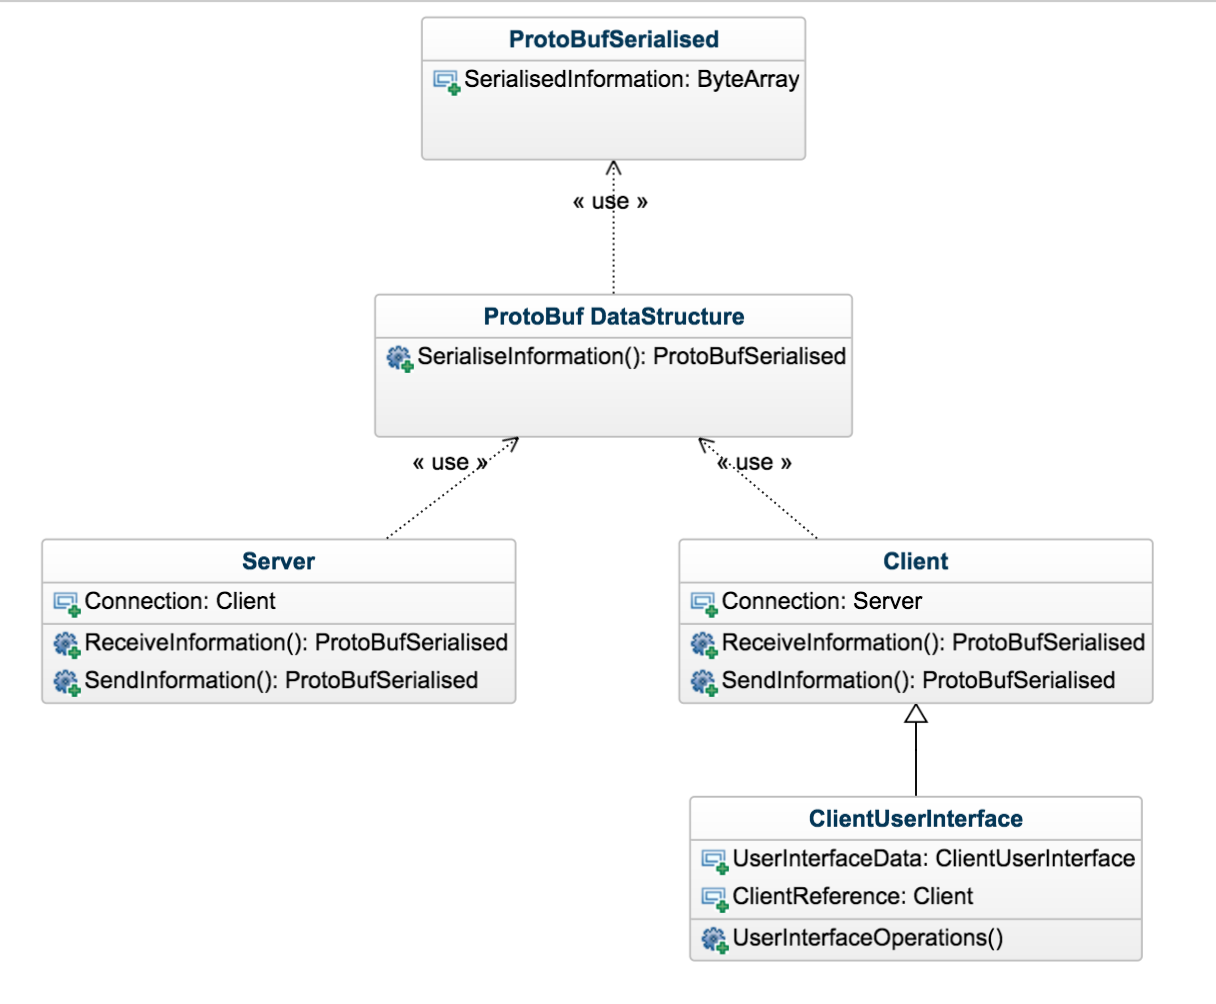
\includegraphics[width=\textwidth]{classdiagram.png}
JominiEngine and its clients have been in continuous development since the project was started, there were more features added on by the students and staff that work on it every year, due to their efforts the development was not starting from a complete scratch and had a codebase with which to work with in order to produce the implementation. David Bond\cite{DavidBond} originally created a single player game with which the work of Helen Rankin\cite{helenrankin} added a networked element, Helen Rankin made a lot of design decisions during the implementation such as designing the protocols with which communication with the server is performed or choosing the libraries with which packets are serialised. Helen Rankin also left a barebones communication interface, this allows for Protobuf data structures to be sent and received from the server over the Lidgren UDP protocol. The above class diagram describes the overall structure of the project, during the development of a client, depending on the platform, the task involved implementing everything but the server. The user interface, whether it be textual or graphical, drives the client, providing the information with which to fill a request with, the request's representation before it is sent to the server takes the form of a protobuf data structure, which using the methods built into the Protobuf framework, serialises this information for transmission to the server. The server receives the information and de-serialises the information from a byte array back into a Protobuf data structure, using the values in the data structure to make the changes to the game state required.
\subsection{Text Client}
The first client implemented was the command line text client, this was chosen first for a few reasons. Firstly, after its completion it would provide a point from which to test the facilities of the server were working correctly, if unexpected results were obtained from running operations from the text client the code of the server relating to the operation that was being performed could be checked to ensure it was working as laid out in David Bond’s thesis. Secondly, the command line client is the least computationally demanding of the three to run, this means that in a demonstration environment this client can be run multiple times on the same machine within virtual machines to test the limits of the amount of connections to a single server at once. Thirdly, the command line client is a C\# based client, this means that the operations codebase, the actions performed after a user has given an instruction to perform via the command line interface can be converted into a Class Library, then compiled into a DLL file for use in different clients written for the same platform, an example of this is the Gtk client provided in this project. The text client is written with little library support, this means that is does not have the baggage of, for example, a graphical user interface library through which it must process every operation. This is adventageous for the portability of the codebase in the sense of re-using code and also with regards to the platforms on which the code can be run, by implementing a multi-platform, modular codebase first this gives a huge platform from which to extend from when building more clients in the future. 
\subsubsection{Build Pipeline}
To produce a working client a build pipeline had to be prepared, this involved the creation of a shell script which ran through the build process that was required depending on the system if it was currently running on. If this is a Windows system the ‘msbuild’ command must be called on the required .csproj files, if it is a Unix based system such as Linux or OSX it is required to run the ‘xbuild’ command, this is the Mono version of msbuild and it takes the same arguments. Both Linux and Windows compile to executable files which can be run as would a standard executable from command line, the path to the file is passed such as ‘./path/to/executable.exe’, however Mono on OSX requires the file path to the executable to passed to it via the mono command, to run the same file the command ‘mono /path/to/executable.exe’. To produce a shell script which could be run on any platform by a user of any skill a build script was produced, this compiles the latest version of the codebase and then runs both the server and the client with the correct commands depending on what operating system the user is running.
\subsubsection{Modifications to Server Code}
The server code the study inherited had some compatibility issues when running on systems other than Windows, mostly relating to file path errors. An external Windows server is probably the best choice throughout the testing process but during the development process access could not be obtained to a machine running the correct configuration and there was a need to be able to attach a debugger to the server to see the information it was returning depending on the messages the client sent to it no matter which system it was run on, to achieve this some changes to the server code were needed. This required to make different decisions based on which file paths were used when accessing log files and security keys based on the type of system that it is being run on.
\subsubsection{Structure of Program}
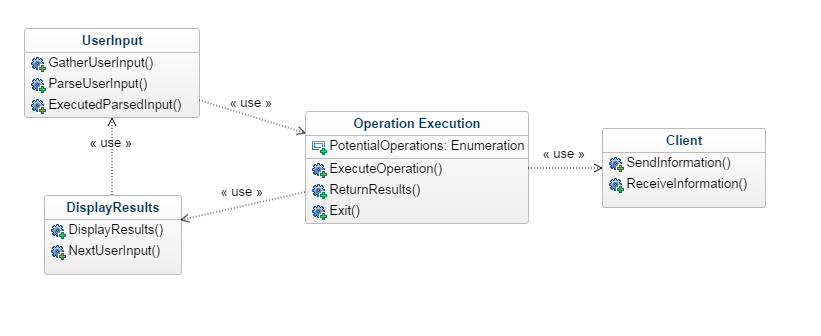
\includegraphics[width=\textwidth]{textclient.png}\\
 The text client works in a loop, it takes user input, processes it and then based on the input it receives it executes a function. The execution of the function makes use of the communication layer, this contacts the server with the user supplied information and then awaits a reply, when the server replies it then hands the information to the display class which in turn sets the client up for the next input from the user, this continues until the program is shut down or the user types the exit command. The program attempts to remain as modular as possible, decoupling of the processes for the identification of user input, the execution and networking layer means that code is easier to re-use in later instances, this makes for less error prone and faster development. The decoupling is key, in order to achieve the goals of modularity and extensibility set out in the project's aims, to provide a platform for future JominiEngine clients to piggyback off the codebase must remain as maintainable and as modular as possible. The lack of library usage in the text client provides a perfect beginning for the creation of more clients, the structure and make-up of the text client is a client in its simplest form.
\subsubsection{User Input Processing}
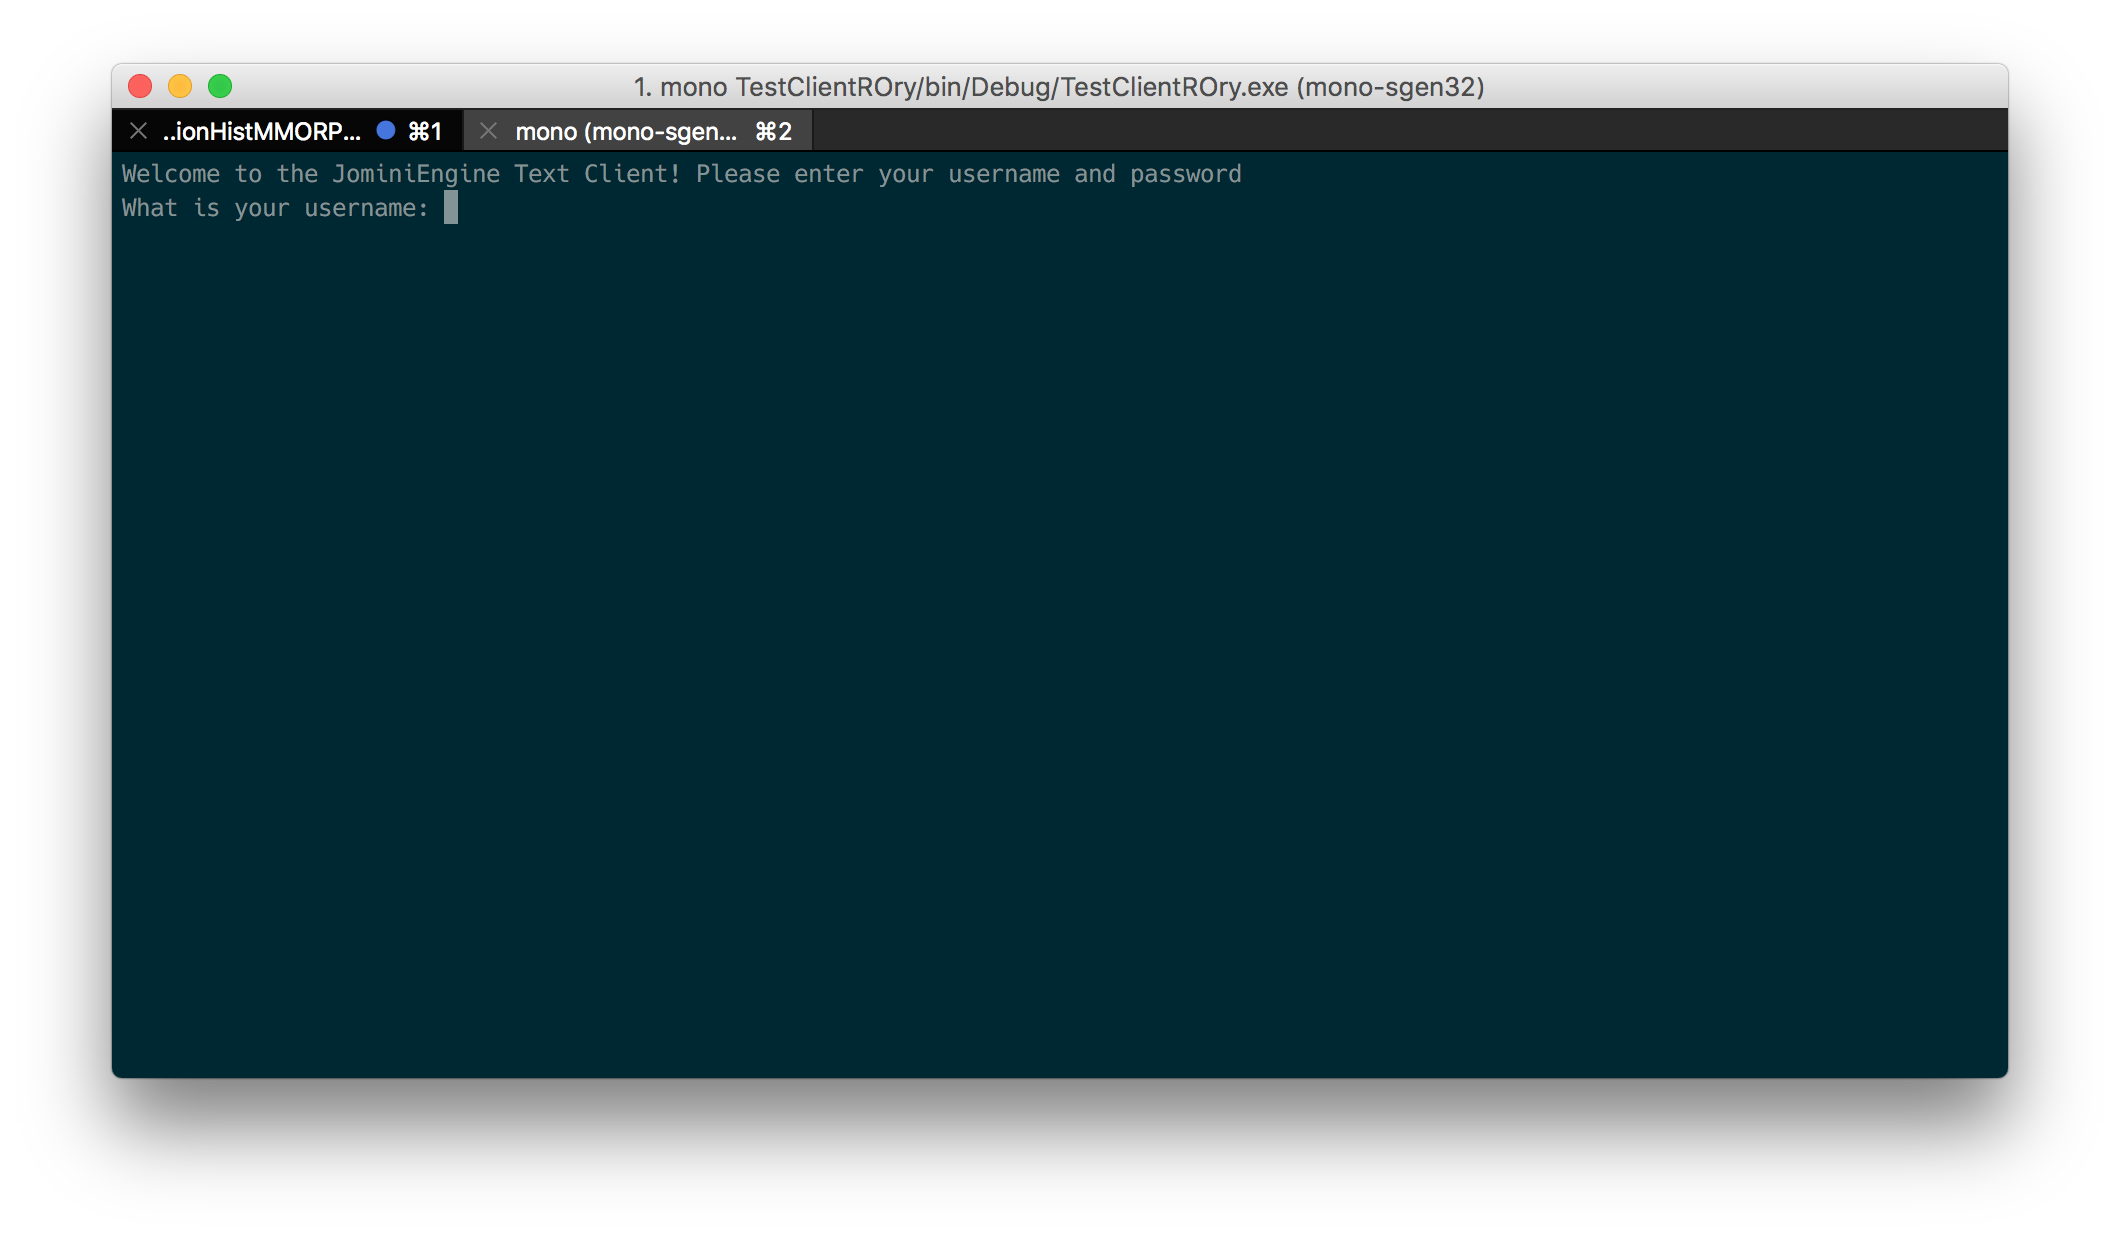
\includegraphics[width=\textwidth]{text1.png}
The structure of the command line client is split into three main sectors, there is first the part which takes user input in and processes it so it can be recognised as discernible commands with arguments if are needed. This takes place in the WordRecogniser object, which converts command line input into a UserOperation enum value, every command has a value in this enumerated type which corresponds to it. WordRecogniser is also used when a command requires a directional argument such as the Move command, this converts a direction, for example “NorthEast” into the corresponding direction in a format the program can understand. This user input processing is the process which indentifies which of the three areas of JominiEngine the command which the user wishes to execute lies within, wether it is Army Management, Fief Management or Family Management and within the context of the client if more than one of these functions can be required at one time.
\subsubsection{Operation Execution}
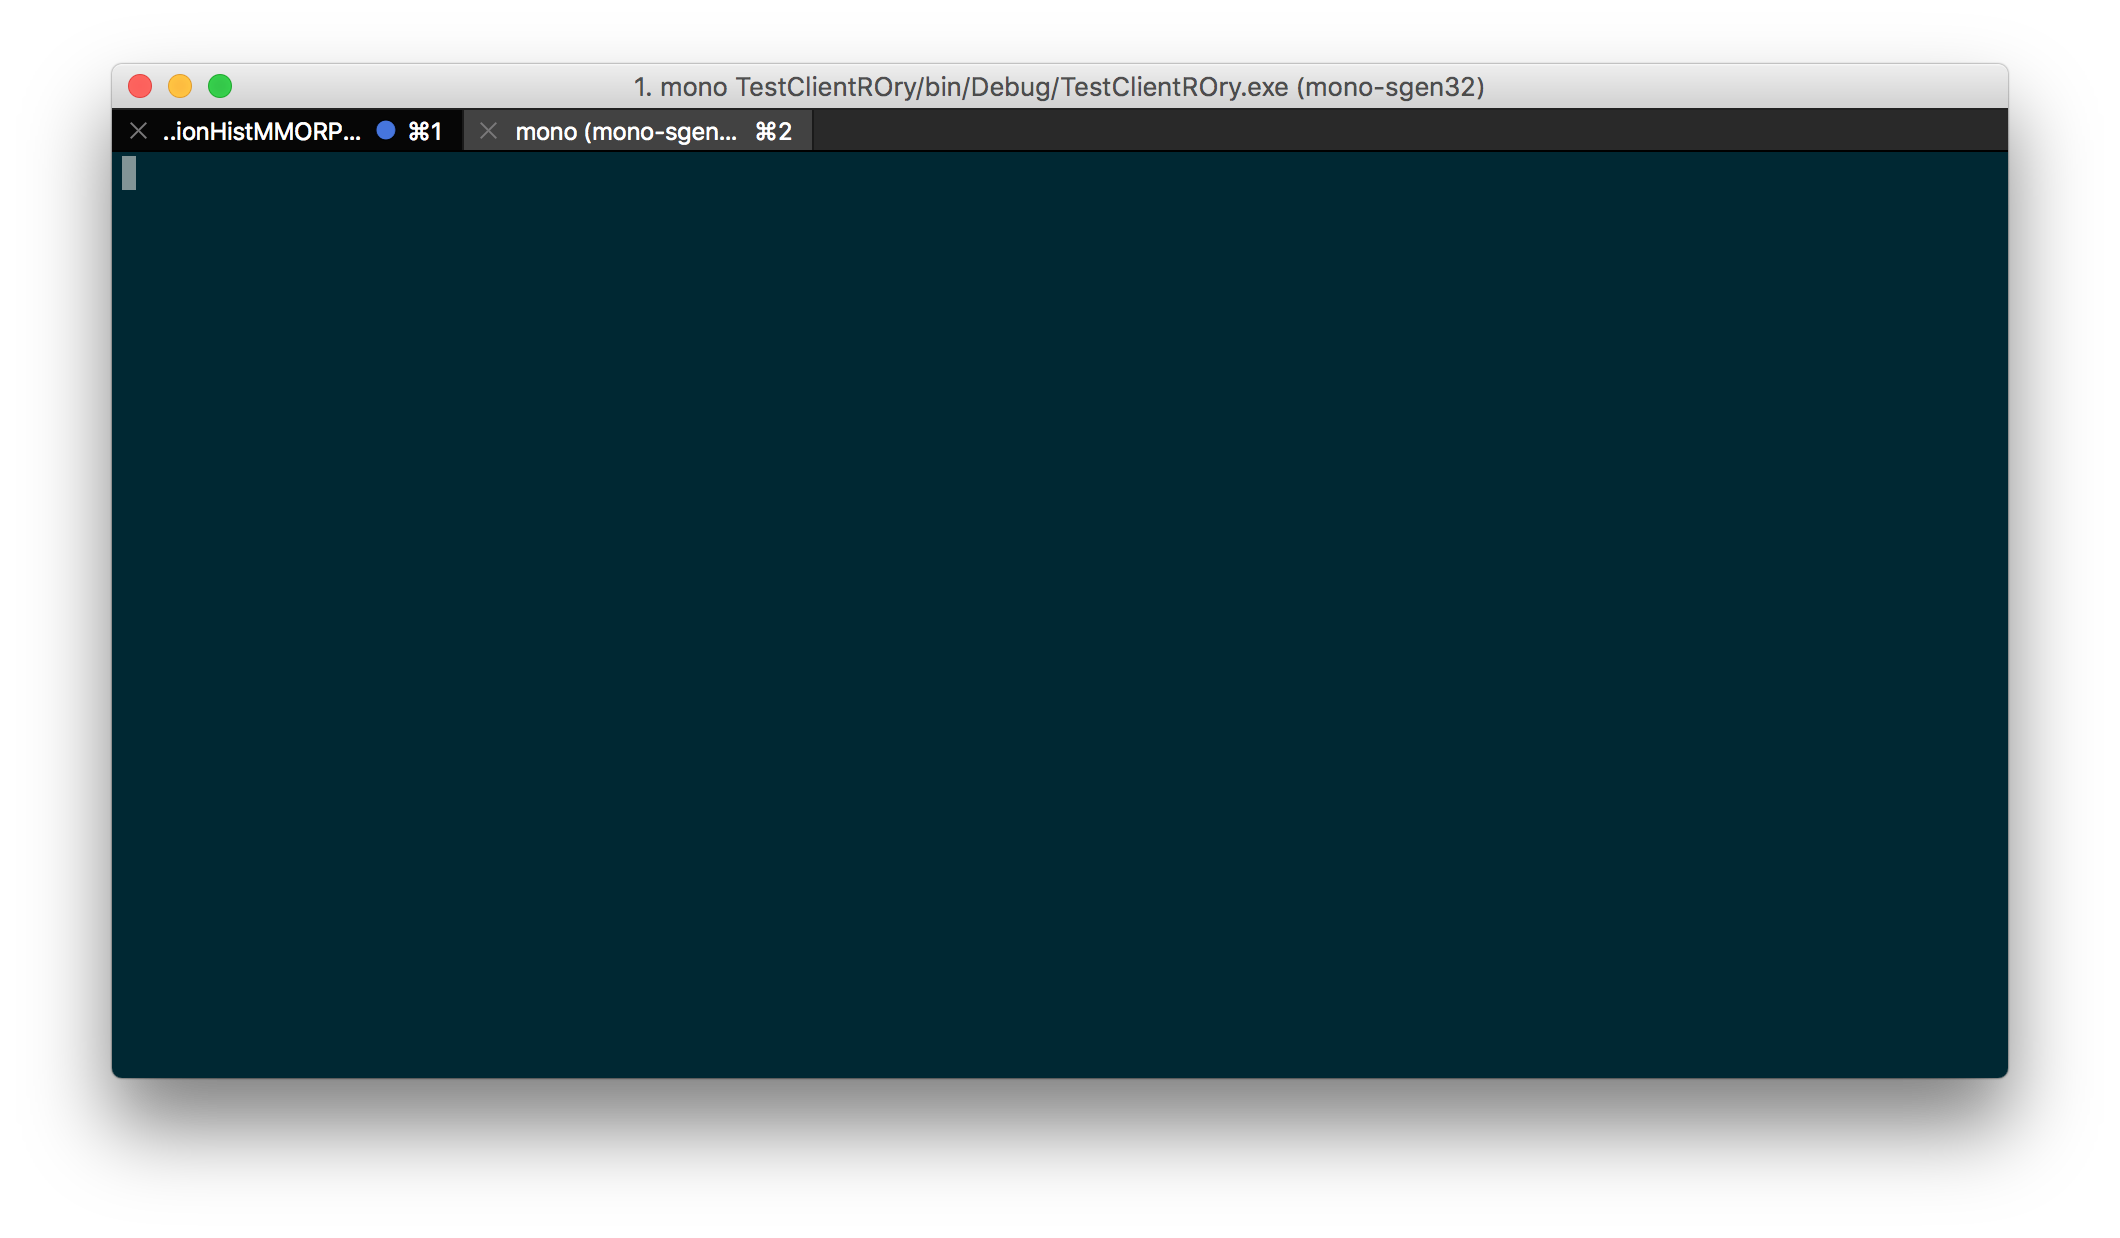
\includegraphics[width=\textwidth]{text2.png}
After the processing of the input occurs this is handled off to the required process in the PlayerOperations object, this object is the object which is abstracted out at a later point into a class library for use in other clients in the future, the program specifies which method it wishes to call and the PlayerOperations object sends the request to the server and returns the reply in a readable format. For example, if the player wished to check the contents of the current fief they would type the command “fief”, this would then be processed by the WordRecogniser object and that would specify a fief operation needed to be performed; PlayerOperations.Fief() would then be the method executed by the program which would return all the information corresponding to the desired fief as outlined in the ProtoFief object from which was inherited from Helen Rankin’s work on the expansion of SessionTypes into the Jomini engine.
\subsubsection{Displaying Data}
There is then a third and final sector of the command line client which deals with the displaying of data once it has been retrieved; when the client is notified of a reply from the server the result of that reply is handed off to the DisplayResult object, this takes in as an argument the ProtoMessage subclass relating to the command that has been performed and each command has a separate method for displaying the information retrieved from the server in the correct format.\\
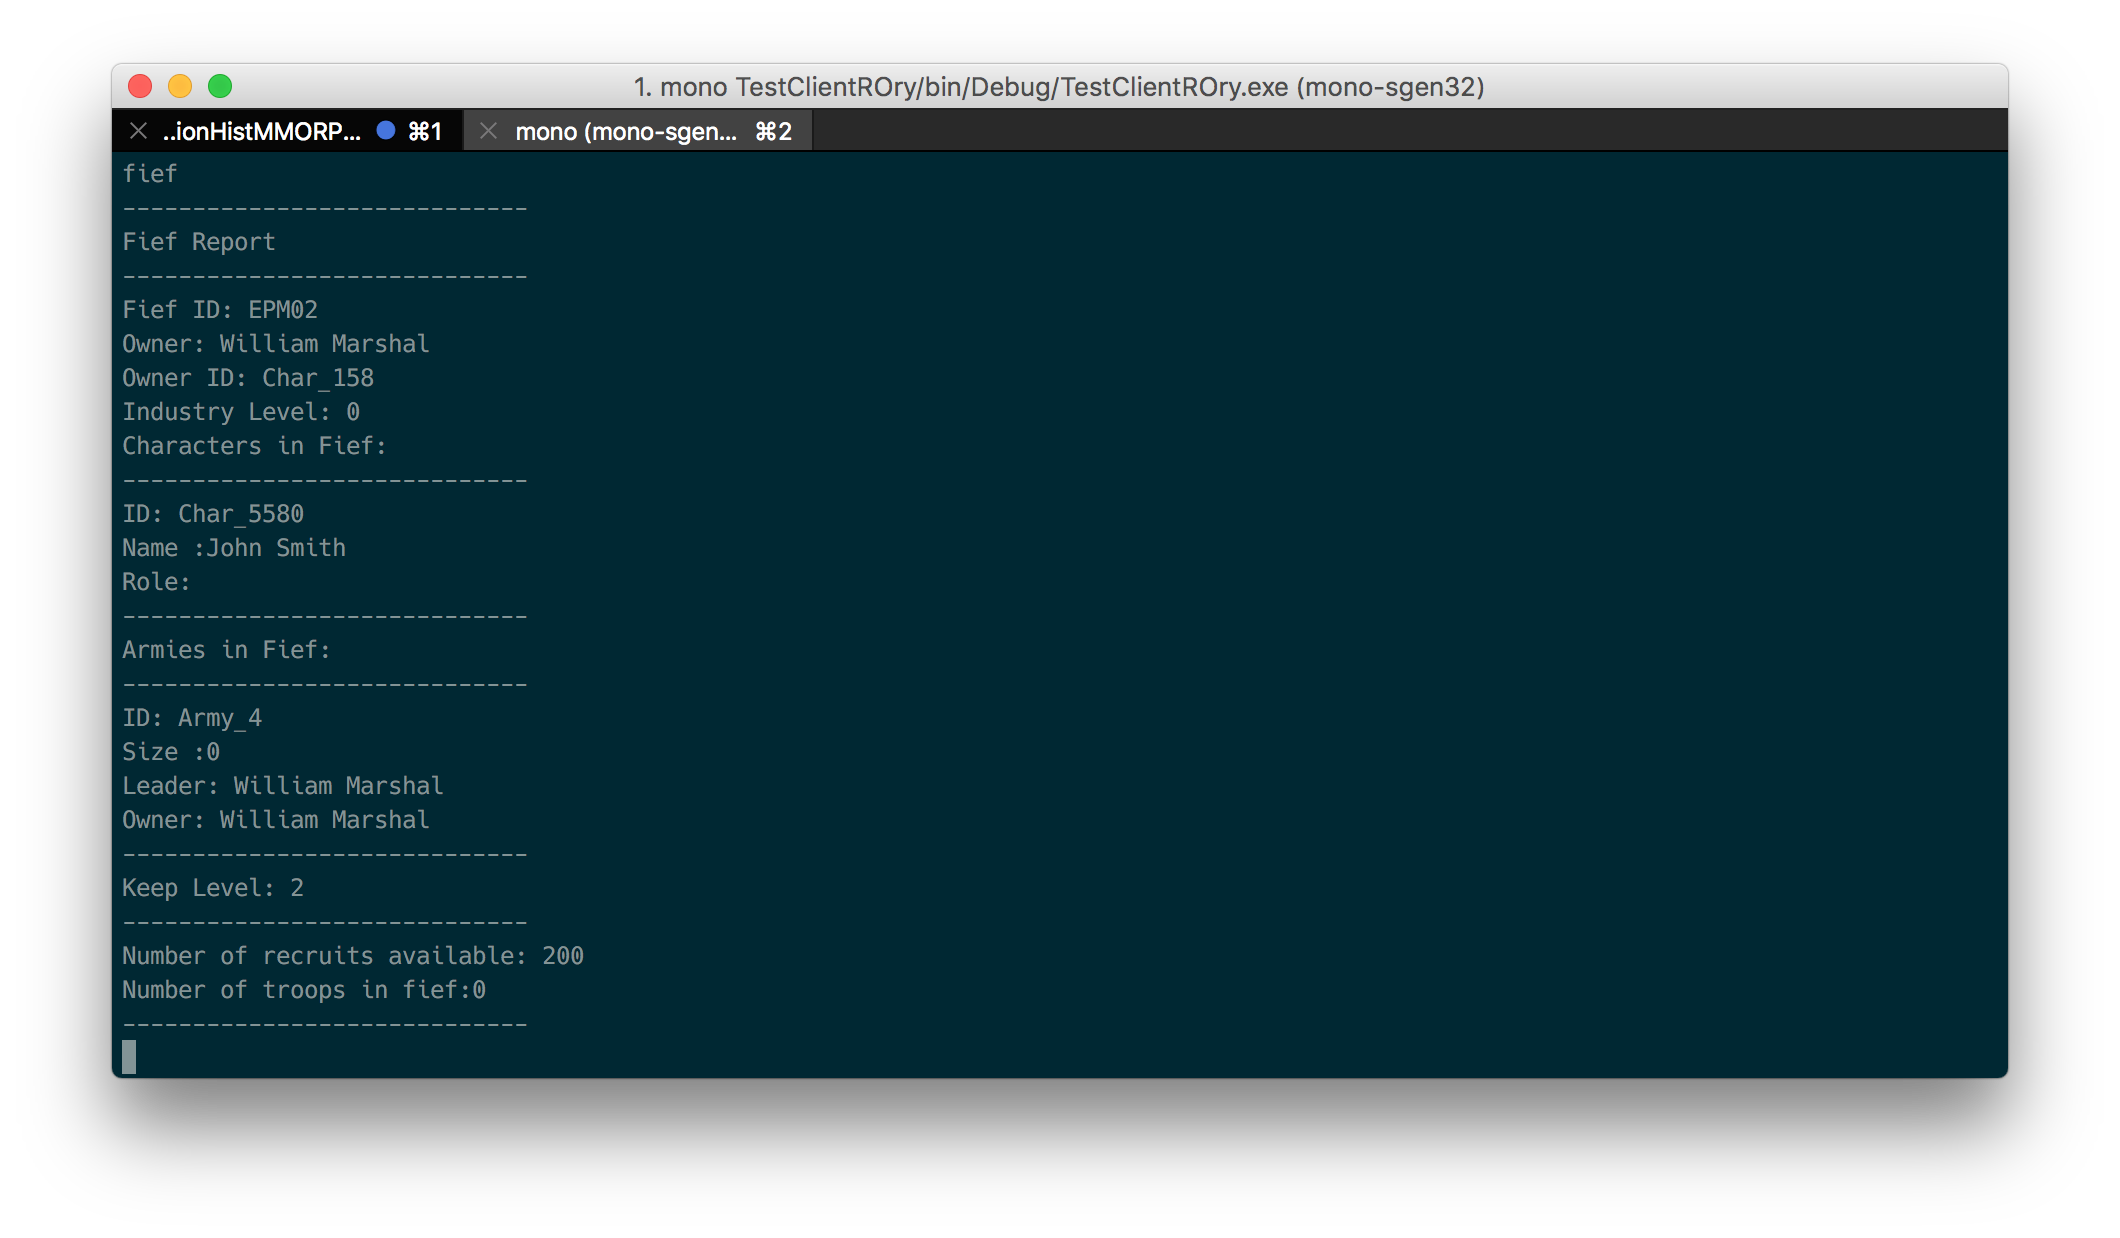
\includegraphics[width=\textwidth]{text3.png}
Above shows the report that a user is provided with if they wish to see information about the fief they are currently in, the report displays a variety of information including the armies currently in the fief, the number of troops available to recruit and the current characters found within that fief. This section of the user interface is a component of both the fief management and army management sections of the JominiEngine game, it allows for a user to gain information with regards to the ability to expand their armies and also about the current status of the fief. While Fief and Army management are functionally disctinct sections of the game the user interface can be contructed to present more than one section of the games utilities to a user at one time. In the context of the user wishing to see all information about a chosen fief it makes sense to display all the information possible, being agnostic of the sections of the game it will involve.\\
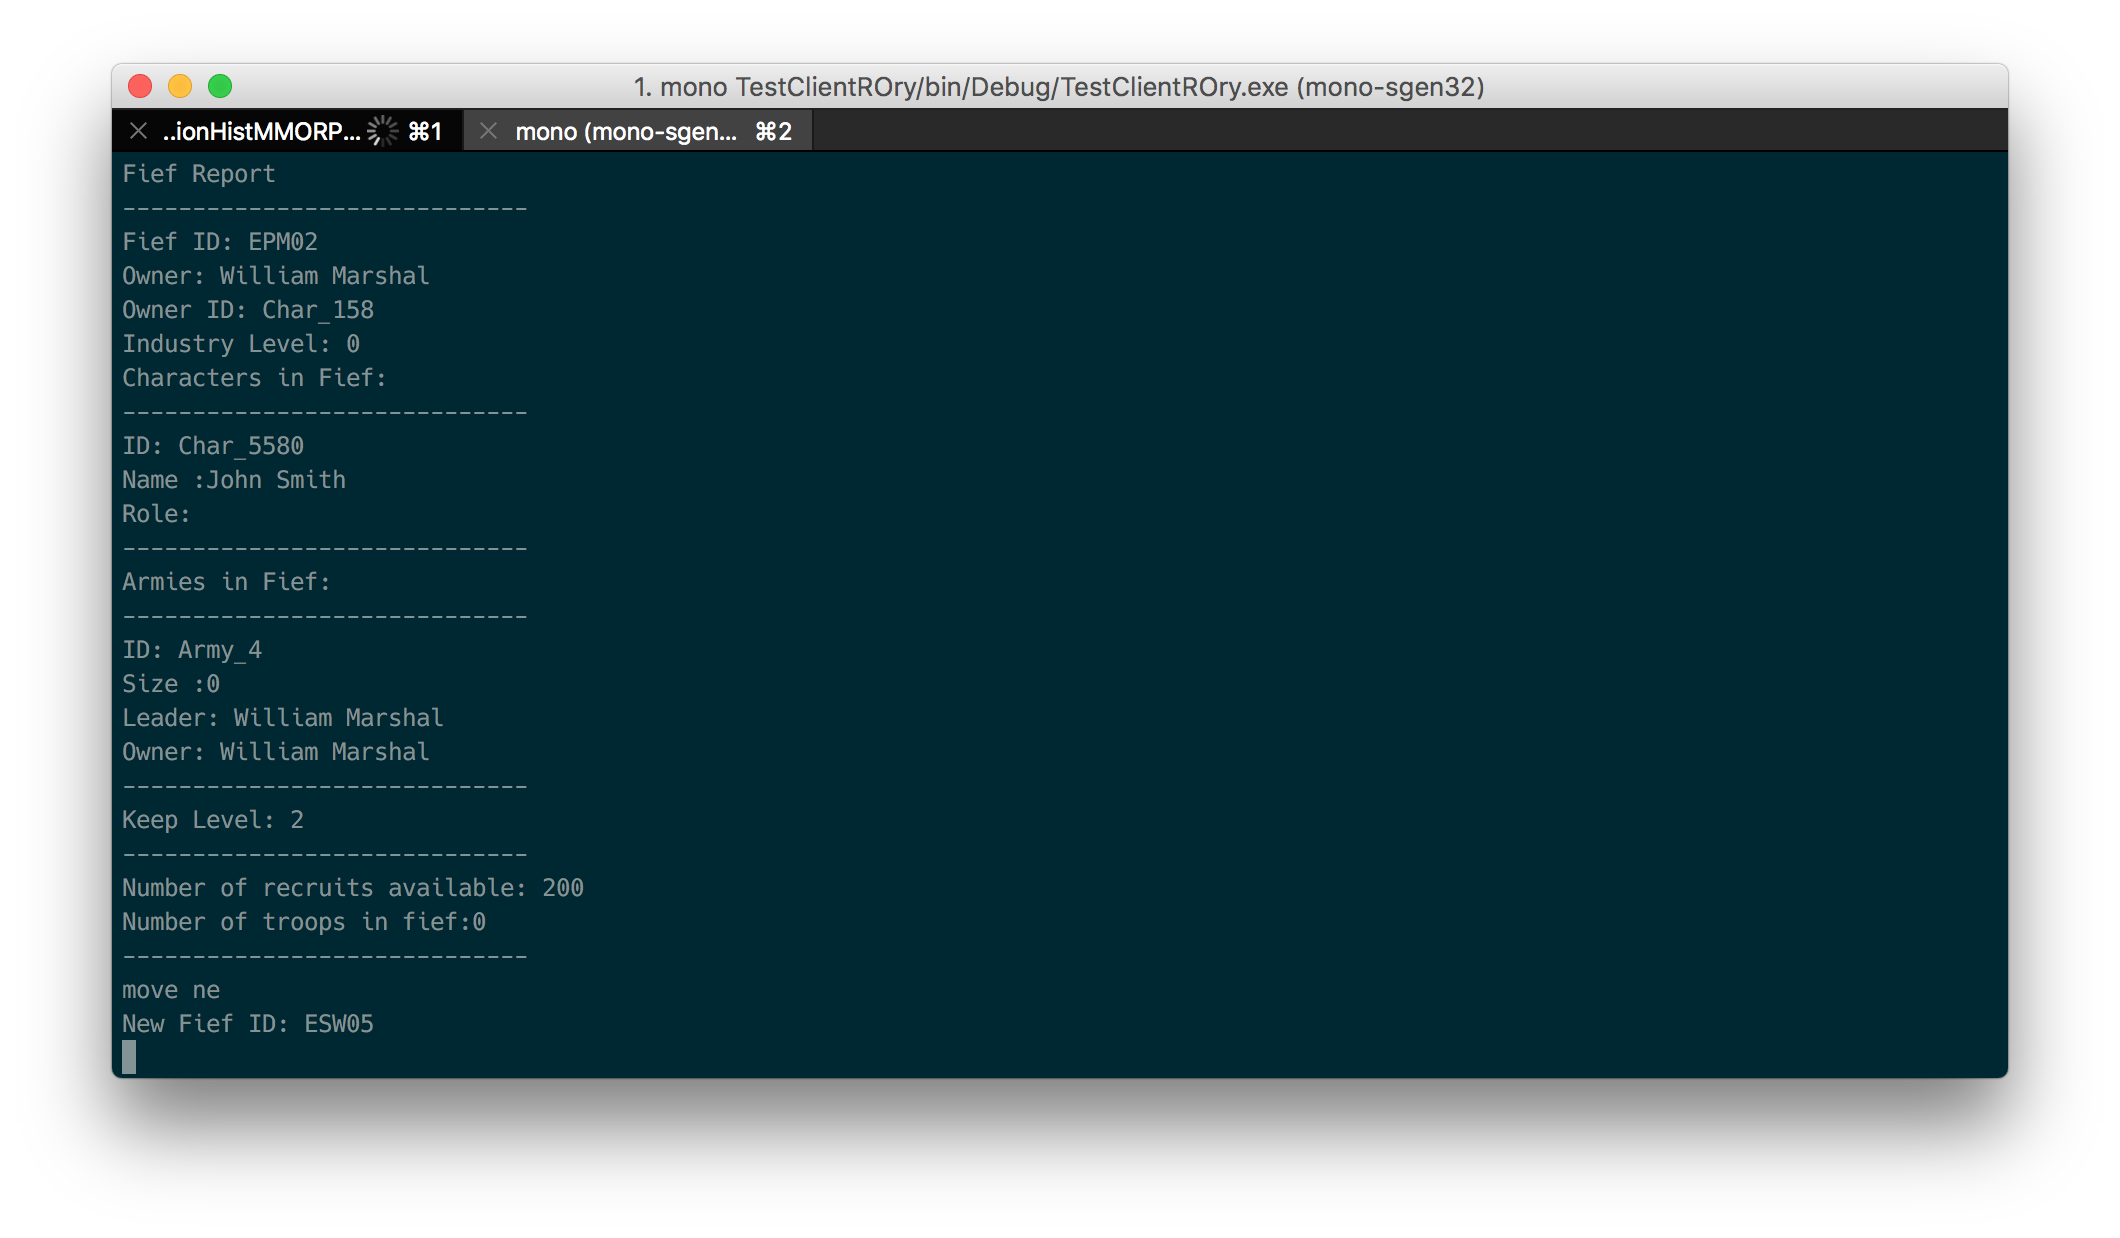
\includegraphics[width=\textwidth]{text4.png}
Above is the output of a move command, a user provides the client with a 'move' command and then supplies as an argument a direction in which to move, this can either be, for example a long hand 'northeast' or a shorter 'ne'. This part of the user interface applies to the Army management section of JominiEngine's operations it allows for the user to transport both their character and army from fief to fief within the grid.\\
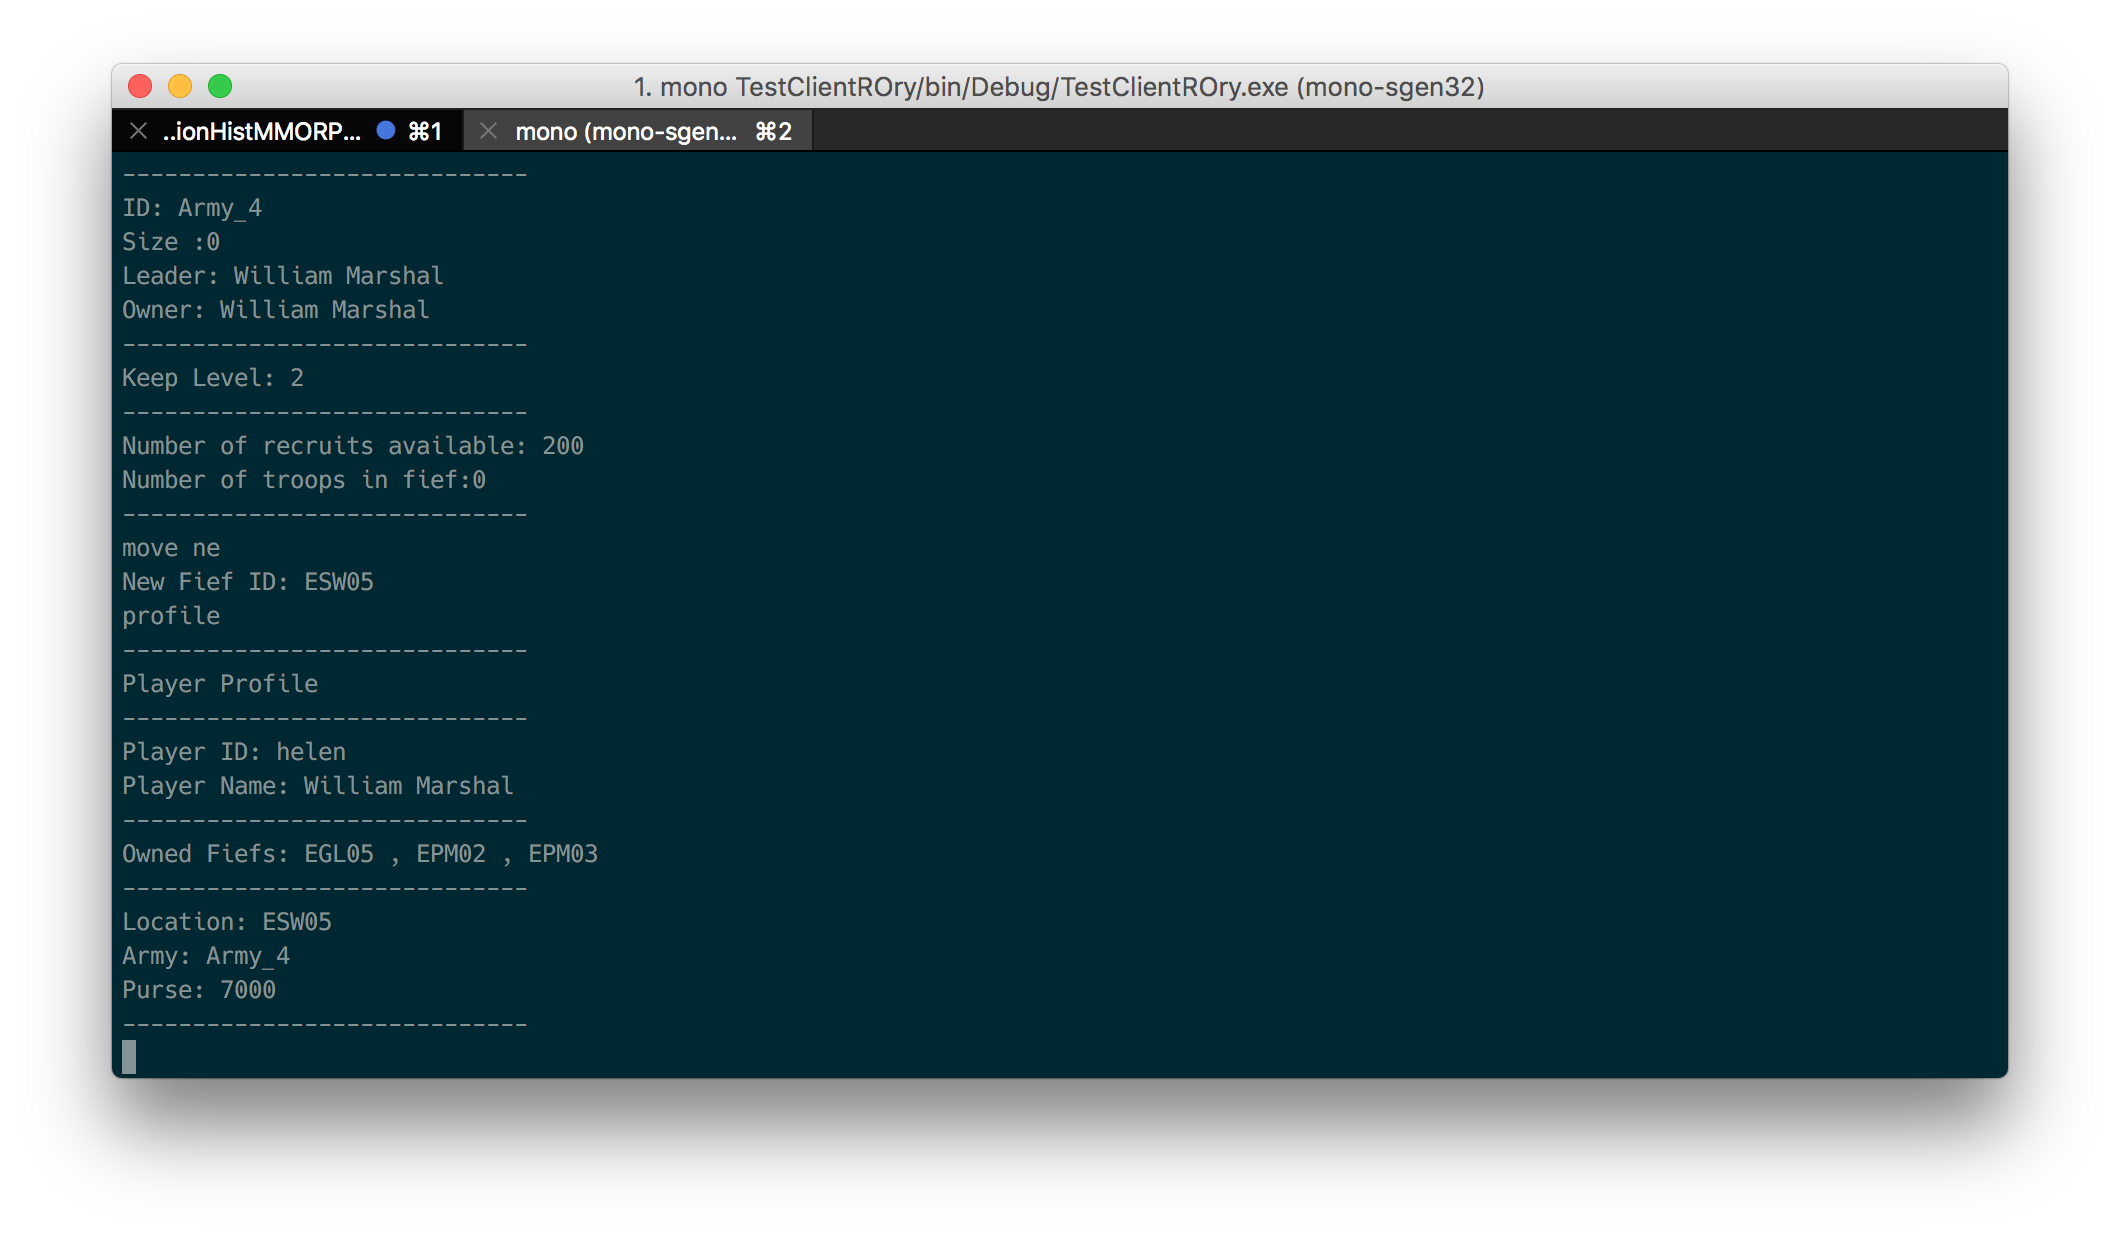
\includegraphics[width=\textwidth]{text5.png}
Thirdly there is the example of the player profile, this returns all information relating to the player's current status, including the fiefs they own, information about their army, and the amount they currently have in their purse. The player profile allows for the user to understand entities that are attached to the character they are currently playing as. They can compare the current status of their character against every entity inside of the system, all items that relate to the player of some sort are displayed to them including their armies and fiefs that they manage, the player profile encompasses every element that relates to the player and the actions they can take.
\subsubsection{Modularity}
A Dynamic-link library is a shared library which allow for programs to take advantage of the resources contained within them by adding them as a project reference, this concept is useful when, for example, developing a client for a game as the communications layer can be used in multiple contexts with different interfaces driving the execution of certain methods within the DLL. A model like this was chosen for the Unity based client, the communications layer built earlier was ported to a class library named ClientDLL which acts as an abstraction and interface for the PlayerOperations object.
\subsection{Graphical Client}
The second part of the implementation required creating a graphical user interface for the JominiEngine client, this client had to have the same compatibility as the text client, running on multiple operating systems. Operating system user interface cross compatibility is a difficult problem to solve and opting to creating such a client limits the scope of your options for frameworks significantly, originally there was an attempt to write a client in the Unity framework, however for reasons that will be expanded upon later int the report this proved unsuitable, in the end the open source Gtk framework\nocite{GTK} was used to create a responsive graphical user interface which ran on multiple platforms.

\subsubsection{.NET Version Incompatibility}

While Unity supports C\# for scripting to some degree, allowing for code to be written which makes use of assets inside of Unity projects to control the scene, attaching scripts to triggers or events which are then executed the version of C\# Unity has support for is not an up to date version, and it is not feature complete. Unity supports up to version 2.6.5 of the Mono cross platform compiler, this is problematic for development, if a project wishes to make use of a library which uses more up to date features of the .NET framework, it can cause a compatibility error which means that importing the library is impossible. Gtk however, is a library which is added on top of or alongside an original C\# project written in whatever version of the language the developer chooses, which allows for the use of more advanced features of the .NET framework. A compatibility issue occurred when trying to make use of the Protobuf data structures in the unity environment, the implementation of Protobuf used by this project’s C\# codebase makes use of a library named Protobuf-net. Protobuf-net makes use of advanced serialisation features within the language to allow for the developer to write the data structures inline using flags explicit to the library to tell the Protobuf compiler how to handle the data stored within the structure. Effectively, this library allows for, instead of writing the protocol in Protobuf’s domain specific language and then compiling to C\#, the developer can write a C\# class and sprinkle it with Protobuf syntactic sugar and reach compliance with the standard there instead. This compatibility error had no solution within the Unity framework, whereas Gtk had no limitation with regards to the language features that could be utilised. One solution which was considered to still use Unity was to extract the Protobuf domain specific language code via the Serializer.ToProto$<>$() contained within Protobuf library, this takes in a Protobuf-net compliant data structure and returns the domain specific language equivalent, and then recompile it targeting an earlier version of the language, however this may have caused errors or incompatibilities with regards to data structure signatures faced in the implementation of the Android client as is explained in section 3.5.4, ultimately this problem meant there had to be a move away from Unity. This required a look for other solutions to producing a graphical user interface, the support that Gtk offered with regards to language compatibility made it a solid choice. Unity has a large support community which provides a host of documentation which was the original reason for picking it as the potential candidate for implementing the User Interface, however, Gtk sees cross language support and is used heavily within the Python community as well as the C\# community. Gtk’s wide, cross language, cross platform userbase provides a host of documentation and guides which sped up the knowledge gathering and then development process.

\subsubsection{Inexperience with Unity}

Another problem encountered when carrying on with the development of the client using the Unity framework was the general inexperience with the platform. While with time, a client that used Unity could have been produced it is much more complex than the Gtk, the tool finally settled on, to get grips with and produce a prototype. As time constraints towards the end of the project closed in and the errors with Protobuf versioning compatibility started to arise and prove themselves to be a formidable tasks in itself to get to grips with and mitigate, the decision was made to use Gtk instead.

\subsubsection{Gtk Implementation}

Due to Gtk’s cross language and cross platform compatibility there was already some experience with it via building user interfaces for a Python program, this was valuable knowledge, after setting up the Gtk build pipeline and getting to grips with the differences from Python it allowed the development process to get up and running much faster than if Unity had been used instead. The portability of the structure of the text client made it so a lot of the communication layer was already complete, the user interface structures to drive and display this information needed to be built around it.
\subsubsection{Structure of Program}
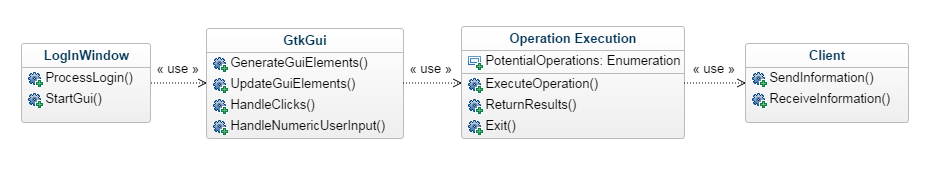
\includegraphics[width=\textwidth]{gtkclient.png}
The Gtk client has a similar program structure to the text client, however the loop that is implemented inside of the text client to capture user input is now captured within the Gtk framework. Gtk allows for the programmer to attach certain functions to event handlers, such as on a button press execute this function, this means that the functions for carrying out operations are matched to the relevant button, and include the code for displaying the relevant information inside of this. On a button press, Gtk captures the event then executes the operation on the client which then waits for a response from the server and returns the result via the mechanisms described in the rest of this section.

\subsubsection{Display Grid}
Gtk offers many tools with which to build usable interfaces, however, a single window can only display one object within it at a time, therefore, a grid must be created in which to store multiple objects to display to the user, this grid is then added to the main window from where the user can interact with all the facets of the system. For our implementation of JominiEngine, there is an overarching table which all display information is stored within, this includes multiple individual tables such as the profile information table which is re-constructed every time an operation is performed by the user. This display grid compartmentalises all elements of the user interface and allows for a developer to target individual elements of the it for update, an abstraction from creating a new window with a new mark up every time an update is triggered.

\subsubsection{Profile and Fief Display Classes}

The information on the player, their armies, and the fiefs they visit updates frequently, a robust model, in this place an object, must be in place to display this information to the user. These classes must mirror the details within the respective protobuf datatype and have the mechanisms to take this datatype and from it construct a user interface which can be displayed. To represent the user’s profile, for example, the program must consider the information stored within it, this consists of the user’s character ID, the user’s character’s name, but also contains more complex information such as an array of all the armies currently under that user’s control. The best mechanisms to display this information, native to the tools that Gtk give us, are to place them within a table grid system, therefore the display classes must take the information as input, via their constructors, and then compile them into a grid, which is then returned higher up the UI stack. Since the information in the grid is not always the same size or in the same format, for example, some users have more armies than others,  an exact one to one reference which is easily updatable cannot be kept, it is impossible to keep a single label called “ArmySize” in which the value is updated as the user hires more units. Therefore, whenever there is a wish to update the value of a the profile or the fief information display, it is required to destroy the old object and create it again with the new information added in via the constructor. To destroy the old information the Destroy() method must be called upon the old object, this initiates a garbage collection upon the object and removes it from the user interface, this is performed from higher up the user interface hierarchy via a method, DestroyProfileTable(). After the object has been cleared redraw it by creating a new object with the information from the request to the server, this is performed on the fief display every time the user sends a move command, updating the information about the fief the user is currently in.

\subsubsection{User Interface}

As mentioned before Gtk makes use of objects named “windows” which are allowed to contain one UI element each. Windows as a function are useful when creating sections of the application which are markedly different from each other, an example of this is the login screen during the setup process of the application. Since the user's login credentials are needed in order to fetch information relating to that user's character, before a login in has occurred no information can be displayed to the user, the user interface, its display grid and fief and profile display structures would be empty. Have a skeleton of the application with no information loaded into it is confusing for the user and bad for usability. Therefore, making use of windows, a login in screen can be generated which is displayed to the user when they first run the program 
\begin{center}
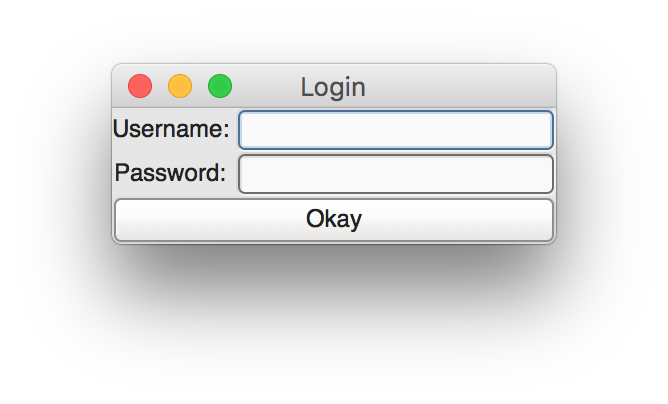
\includegraphics[scale=1]{gtk1.png}
\end{center}
This login screen prompts the user for the correct information with which to proceed, when the user has completed this task they press the ‘okay’ button to continue, there is no other possible path for them to take. When a user completes this task the login occurs and the server fetches the information which is relevant to their profile, this is then presented to the user via the display classes described earlier.
\begin{center}
	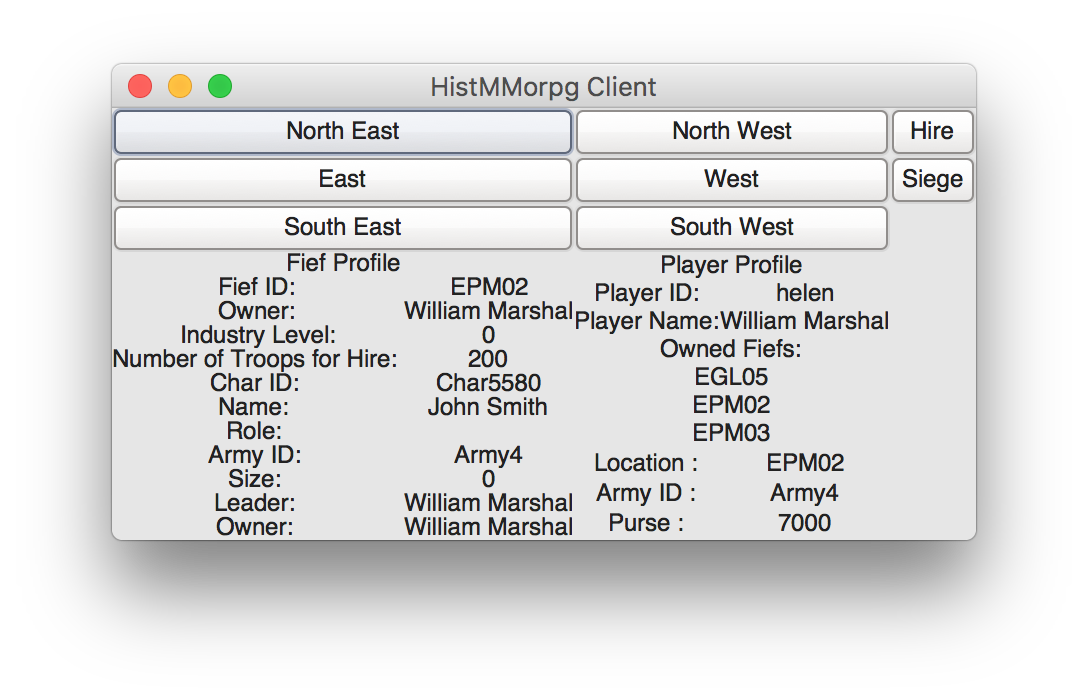
\includegraphics[scale=.8]{gtk2.png}
\end{center}
Within the main window of the graphical client the user is presented with the utilities with which to access all aspects of the JominiEngine player's functions. They are presented with the directional buttons arranged aligning with the compass axis to which they correspond, if a user clicks one of these buttons they and their army are transported in that direction. The user also has the possibility to recruit soldiers if they have the funds from fiefs which they are in control of and have recruits that are available, an error message is returned if these criteria are not met. The user also has the option to begin sieges on fiefs which are controlled by an enemy player, they use the army they have transported to the enemy fief they currently reside within to begin a siege, the results are then reported back the user. If a siege is unsuccesful and a player's controlled character is killed, the player then assumes the role of the characters descendent if one exists, this fulfils the family management role of the JominiEngine gameplay.
\subsection{Android Client }

Natively Android supports the Java programming language, which it then compiles into an Android specific bytecode for execution on the Android runtime. User interfaces are designed via an XML compliant domain specific language, these are then loaded into runtime and referenced within the code and are manipulated via this reference. The Java runtime environment runs bytecode and therefore other compilers for languages other than Java have been created, the most notable of these is Xamarin which allows for C\# code to be compiled targeting Android runtime bytecode and then the program to be executed in the same way as a native Java application.

\subsubsection{Android Networking}

Android applications are limited in the scope of access to the device’s hardware they are entitled to via the permissions the user allows for an application to run with. These permissions, included access to the android device’s networking stack, are compiled into an xml file in the project’s root named manifests.xml; since the application makes use of the networking stack, there is a need to inform the user of this before the application runs. Since the Android application runs inside of an emulator, the game server is hosted on a different machine to that of the client, this means that connecting to localhost where the game server is running is not possible. The Android emulator comes with a built in solution to this in the form of the reserved IP ‘10.0.2.2’, this address is an alias to the host machine’s loopback interface and allows for the emulator to access the host machine’s localhost.

\subsubsection{Communication Protocol}

Helen Rankin's\cite{helenrankin} server implementation made use of the Protobuf-net library for C\#, this is useful in that context as it allows for the developer to create the Protobuf message formats in native C\# with syntactic sugar added that the compiler can understand when the build process is executed, compiling native C\# objects for use on the protobuf layer. However, Java does not have a similar feature, it requires the Protobuf data structure to be written in the Protobuf domain specific language, and if it did there would need to be a re-writing of the Protobuf data types in Protobuf-net to the Java equivalent, this proved problematic, a solution had to be devised which avoided this time-expensive process. The C\# Protobuf library's Serializer.ToProto$<>$() method was used, this method within the Protobuf-net library takes in a data type, in this case, the ProtoMessage superclass of all the Protobuf data structures in the C\# client implementation of JominiEngine and produces the Protobuf domain specific language implementation of the Protobuf-net C\# data structure. Once the output of this was saved to file, the result could then be run through the Protobuf compiler with a Java compilation flag to produce a Java file called HistMmorpg.java, this file contains a Java implementation of the Protobuf-net C\# data structure used in the text client ready for use on the Android platform.

\subsubsection{Networking Interface}
In order to communicate with the server the networking stack inherited from earlier clients for sending messages between the client and the server had to be re-implemented. Originally this re-implementation began in Java, however due to some issues explained later the passage with regards to compatibility the decision was ultimately made to move the project to a Xamarin based solution for Android. This included an implementation of the packet sending mechanism inherited from Helen Rankin's\cite{helenrankin} work on session type based networking to the server, the players username is added to a packet in its byteform and the string "TestString" is then appended to the byte array. This creates a packet which matches the specification outlined in the server code for accepting a new connection from a user, once a packet matching this form is sent to the server a connection is accepted, this then opens a channel for ProtoBuf data structures to be sent and replies to be received between the client and the server. This code is stored within a delegate which is executed on newly spawned thread on application start up, this keeps the operation off the UI thread, stopping any blocking from occurring which would in turn cause the UI to stall.
\begin{lstlisting}[language=Java,breaklines=true,numbers=left,frame=single,title=LogIn Code,basicstyle=\linespread{0.5}]
protected Boolean doInBackground(String... params) {
	pass = params[0];
	clientUsername = params[1];
	try {
	socket.connect(InetAddress.getByName("10.0.2.2"), 8000);
	try {
		byte[] sendPacket = clientUsername.getBytes();
		byte[] testString = "TestString".getBytes();

		byte[] packetCombined = new byte[sendPacket.length + testString.length];
		int counter = 0;
		while(counter < sendPacket.length){
			packetCombined[counter] = sendPacket[counter];
			counter++;
		}
		int secondCounter = 0;
		while (secondCounter < testString.length){
			packetCombined[counter] = testString[secondCounter];
			counter++;
			secondCounter++;
		}
		DatagramPacket loginPacket = new DatagramPacket(packetCombined, packetCombined.length);
		socket.send(loginPacket);
	} catch (IOException e) {
		e.printStackTrace();
	}
	HistMmorpg.ProtoLogIn.Builder protoLogin = HistMmorpg.ProtoLogIn.newBuilder();
	HistMmorpg.ProtoLogIn logInSalts = protoLogin.build();
	} catch (UnknownHostException e) {
		e.printStackTrace();
	}
	return true;
}
\end{lstlisting}
The original server as created by Helen Rankin makes use of the Lidgren networking framework for C\# in order to send and receive messages on both the client and server, Lidgren formats packets in a certain way that is very specific and while some characteristics are shared with normal UDP packets they do not exactly match. There is no Lidgren implementation or Lidgren clone for Java based systems, while Java has socket utilities that provide similar tooling it is not an exact match. This proves problematic when the server is receiving packets using Lidgren’s read message utility as the current implementation does, if a client does not match the Lidgren specification it is viewed by Lidgren as an errored packet and this is rejected by the server. Java’s native implementation of the socket protocol is found in the DatagramSocket object, this is used to send DatagramPackets via the UDP protocol, it does not add any headers to the packets it sends other than the expected UDP headers for configuration purposes. Herein lies the problem with the sending and receiving of packets via Lidgren when not using the Lidgren library’s send method to package information inside a byte array before it is sent, the packet produced by Java’s native DatagramPacket class does not match the Lidgren specification and is rejected and marked as an errored packet even though the byte array that is sent is the same in both implementations. \\
\begin{figure}[H]
	\caption{Packet Diff, Lidgren Packet on top, Java client on bottom.}
	\centering
	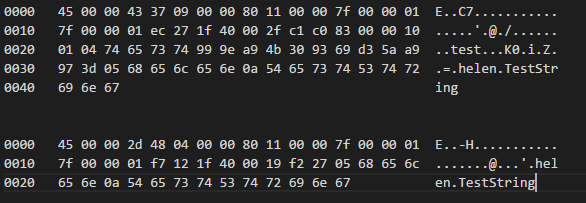
\includegraphics{packetdiff.png}
\end{figure}
In the image above, the original packet sent by Lidgren is the first row of hex text, and the secondary packet send from the Java client using its socket implementation can be seen below, here the differences and similarity between the packets can be seen. Lidgren, at some point, during the sending of packets over the protocol adds extra headers, this includes information referencing the setup process of the client-side NetworkUtlityProtocol object in the client initialisation process. An attempt was made to discover more about the roots of this problem using the Wireshark networking monitoring utility on Windows, this proved problematic due to the fact that Windows does not allow Wireshark to monitor over the loopback address (localhost) where both the server and the client were ran during the testing process. In order to mitigate the issue of not having access to the loopback address RawCap command line utility, which has the ability to monitor the loopback address for protocol traffic was used. RawCap then generates a .pcap file which can then can be loaded into Wireshark for deeper inspection, here the differences between the packets were laid clear and scale of the incompatibility issues was realised for the first time. An attempt was made to carry out some mitigation of this problem from the Java side, including creating methods which formatted a potential Byte array that was sent from Java to include the extra headers for the Lidgren protocol, therefore allowing the server to read the packets this effort proved fruitless, little documentation could be found for Lidgren to help understand and grasp the differences in formatting.
\subsubsection{Development Environment}
The Xamarin framework allows for C\# code to be run on the Android platform under a version of Mono called ‘Mono for Android’. Xamarin also allows for apps to be compiled for the iOS platform with the same codebase, this proves to be very useful when writing cross platform mobile applications. Compared to native Android applications which do not allow for any C\# libraries to be imported in any form, and with the limitations placed on the sending of packets from the client needing to be sent in a format that Lidgren can receive, Xamarin allowed for the development process to make use of Lidgren while still writing code for Android. Xamarin compiles C\# code to the same bytecode for execution on the Java runtime that a native Java application compiles to, functionally the applications appear to the user exactly the same no matter what language they are written in. Mono for Android, however, does not implement the full C\# stack, there are some modifications to the native libraries that are included, for example, the class serialisation utilities are not implemented in the same form that they are in the standard .NET library and the console utilities are left out entirely. The Protobuf codebase and data structures which are used to communicate between the server and the client implement features which do not exist within the Mono for Android subset, they cannot be imported into the application as a reference as-is. While the issues with regards to features which are not available under Mono for Android proved problematic, there are also issues with regards to the types of references that Mono for Android allows to be imported, Mono for Android only allows for the developer to import libraries which are written and compiled to a specific type of DLL, a portable class library. While this required restructuring of the codebase (section 3.5.5) it was still preferred to the native Android implementation which would have required a complete rewriting of the Lidgren library in order to make communication between the clients possible, exporting existing, modular, code from previous clients to a portable class library was a less time consuming and developer effort solution than native code.
\subsubsection{Portable Class Library}
The earlier DLL (mentioned in section 3.3.8) did not match the specification required for a Portable Class Library, and therefore it was needed to construct one from scratch. Portable Class Libraries were added to the .NET platform in 2011 and aim to break away from the restrictions that come with individually compiling DLLs for each individual platform that the program could potentially be run on, when a Portable Class Library is originally created the creator has the choice to mark which platforms it will be running on and the Portable Class Library then enforces the limitations applied to C\# code for all of these platforms to the codebase. In order to create a Portable Class Library which matched the requirements needed, a reference to the ProtoBuf data structures created for the server and client to share and communicate with, code from the server and client test harness created by Helen Rankin had to be brought across. This proved to be an issue, the classes used as part of the Protobuf library are written using the Protobuf-net library which makes use of serialisation features not available in Mono for Android. To alleviate this issue there was a usage of the CSShim library\cite{CSShim}, this makes dummy data structures for use in place of classes used in legacy .NET code which does not comply with the limitations of a Portable Class Library, with the inclusion of this library references to all missing .NET features used were added which made the code compilable but the functionality behind the classes does not exist. The problem with the original JominiEngine codebase is that it is rather tightly coupled; at the heart of it it is a test harness which runs through a method starting a client and a server, leading them through a series of tests of which the outcomes are confirmed and then the codebase exits, the server and client do not operate independently of each other. Furthermore, the server and the client in parts share a codebase, they both make references to Protobuf classes which are in the same solution, they do not import the data structures from a separate solution via a DLL. This is problematic, since the Portable Class Library cannot reference these data structures exactly and has its own versions of the Protobuf data structures which mirror those of the original server and client, functionally and structurally, but with a different signature there is not an exact reference. When calling ProtoBuf methods upon the received packets from the Android client to deserialize them from their transmission state an error occurs due to the fact the data structure that is serialised, although functionally the same, is the Portable Class Library version; the only way to deal with this problem is to reimplement the entire server and other clients using the version of the data structures used inside the Portable Class Library.
\subsubsection{Structure of Program}
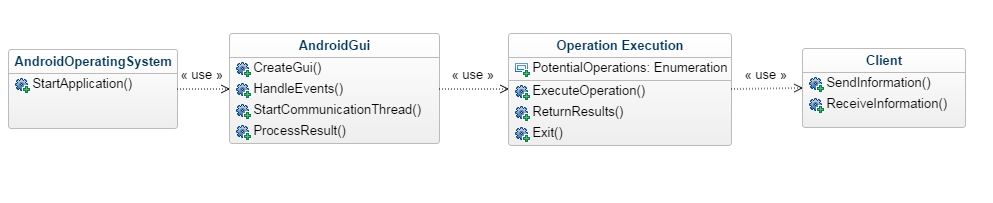
\includegraphics[width=\textwidth]{android.png}
The structure of program that the Android environment allows for is markedly different to the clients before it, largely in the way in which it forces the developer to make use of threading. Networking, which the client makes heavy use of in order to communicate with the server, is completely forbidden by the system from the main thread on which all UI operations are performed in order to reduce the chances of lag occurring. This means that when a button is pressed on an Android user interface, a new delegate is spawned on a new thread from which a response, when it is accessed is returned to the user interface.
\subsubsection{User Interface}
\begin{center}
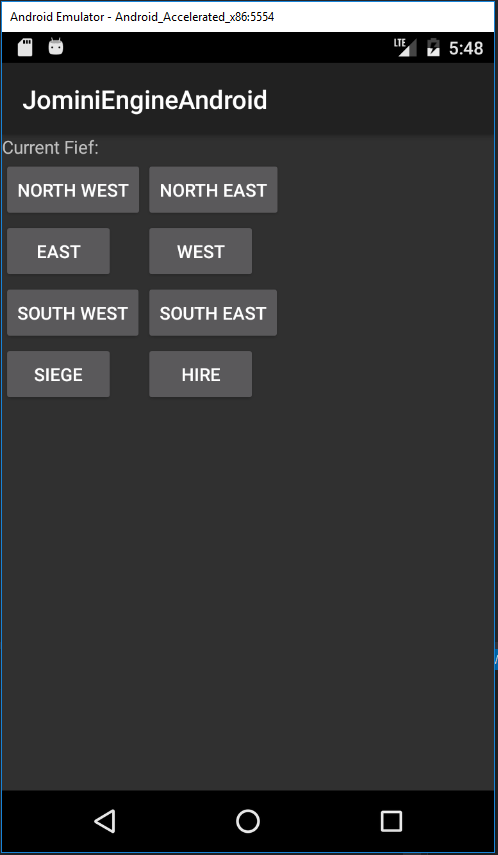
\includegraphics[scale=0.5]{jominiengine.png}\\
\end{center}
The Android user interface replicates a similar one to those that have gone before it, this helps with acclimatising the user to the program. They are presented with movement buttons, laid out in the direction with which the character would move through the map and then further option buttons with which to manipulate the status of their army or fiefs. When they select an option which requires user input, such as hiring a certain number of troops, they are presented with an input box into which the correct amount of troops to hire or other relevant action are entered.
\subsubsection{Completion With Regards To JominiEngine Functions}
Due to the impediment of the progression of the Android client becuase of the need of large amounts of server re-factoring with regards to the data structures used the Android client does not implement the entirety of JominiEngine's functions. At the time of publication the only element of the JominiEngine's core functions that the client implements is Army Management, the client allows for the army to be moved from location to location and for more troops to be hired by the user. It does not allow for sections of the family or fief management functions to be used by the user, while implementation of these functions would be possible, and due to the modularity of the client structure would not require large amounts of changing the application, the fact such large server refactors are required beforehand is blocking the task.
\newpage
\section{Technical Evaluation}
\subsection{Methodology}
The methodology for the investigation into the success of the implementations of each of the clients comes from their technical proficiency. This includes the static analysis of the program which involves monitoring the quality of the codebase as is, without execution and dynamic analysis which requires the program to be executed and the quality of the end result assessed via metrics retrieved from a debugger attached. The methods chosen  to perform the static analysis of the completion of the codebase are built into Microsoft's Visual Studio application, they allow for the user to run a process which generates a 'Code Metrics' table with information regarding the Maintainability Index, the Cyclomatic Complexity, the depth on inheritance and the degree to which the classes are coupled together. The Maintainability Index is a number from 0 to 100, a higher number means that the codebase is deemed by Visual Studio's analysis tool to be 'more maintainable', the Cycolmatic Complexity explores all possible code paths for the flow of the program, more complex programs with a larger logic component will have a higher value. The depth of inheritance is a reference to how many levels of inheritance the codebase has within it, if a there are large numbers of parent classes this will be a higher number, and the class coupling suggests the degree to which the classes are dependent on each other, more coupled code is more difficult to change at a later stage. Due to the nature of the ever evolving development of JominiEngine it is important that the project has maintainable, extendible clients and it is important that static analysis is performed in order to understand the current state of their implementations with regards to potential extension. Dynamic Analysis provides a window into how the program performs while it is running, this is performed by attaching a debugger to the process and observing how the program effects the computer's resources; this could, for example, include the monitoring of the programs memory footprint, or it could look at how many clock cycles an operation takes, the criteria of this is different for every client, the text client must not be demanding on resources to allow more than one instance to be run at the same time, and the Android client must not be memory intensive on a device which does not have access to as much RAM as a desktop machine. The solution for the execution of dynamic analysis finally settled upon is a tool named the 'Windows Performance Analyser', this is a tool that was created for Windows 8 which allows for the user to record the operations carried out on a machine over a certain time period and generate a log file. This log file contains information with regards to various sections of the systems resource, what API's have been called by programs, how much processing power program's made use of and the memory usage of each thread and process. From this tool, graphs can be exported and measured against each other, the results will show how much more of a demand the individual clients place on a system. It is only through the dynamic analysis process that insight into the platform-suitability of each of the clients can be gained, and in turn, if they have completed their goals.
\subsection{Text Client}
\subsubsection{Static Analysis}
Using the analysis utilities built into Visual Studio on the text client project a set of results can be generated that provide us with information about the quality and extensibility of the code base. The text client has the simplest grounding of all the implementations, the overarching functions that it relies upon are relatively simple and do not require extensive library support or the usage of complex language constructs. The client is modular, with each section of the pipeline separate from the other, meaning that the code can be re-used in future projects, this should mean that the code is maintainable and avoid tight coupling. The problem area of the codebase is the display mechanisms, this requires the importing of data structures and console tooling that is not required elsewhere in the solution, it remains more tightly coupled than the other sections of the codebase due to this reliance.
\begin{table}[H]
	\centering
	\caption{Text Client Static Analysis Results}
	\label{my-label}
	\begin{tabularx}{\textwidth}{|X|X|X|X|X|X|}
		\hline
		\textbf{Application} & \textbf{Maintainable Index} & \textbf{Cyclomatic Complexity} & \textbf{Depth of Inheritance} & \textbf{Class Coupling} & \textbf{Lines Of Code} \\ \hline
		Player Command Parser and Execution & 77 &      114     &     1      &    37       &     247      \\ \hline
		Results Display & 59 &       28    &       1    &     13      &       150    \\ \hline
	\end{tabularx}
\end{table}
Since the text client is a relatively bare-bones implementation it provides a good yardstick with which to measure the capabilities of the other clients, using the figures from the results of the analysis allows for questions to be asked with regards to what degree user interface libraries add complexity to the solution, having something comparative allows for conclusions to be drawn on the trade-off of increasing the complexity of the client.
\subsubsection{Dynamic Analysis}
Dynamic analysis involves the monitoring of the program as it is being executed, with regards to the text client it aims to be a low cost client which does not require significant processing power to run. Throughout all the tests the constant running of the server executable gives us a benchmark with which to compare the cost of running a certain client, the server should overall, throughout all the tests, record the same average processing power usage, the cost of running a client can be compared to the average of the server to work out which client is the most demanding. In the case of the text client the below graph shows the 'weight' of running the program, weight is the percentage of CPU time in that instance that is execute the program. In the below graph the server is the yellow line and the client the blue, it can be observed that as the client sends a request just before 9 seconds the server receives the request and then responds, the client then displays the value in the return, causing the spike in activity.  \\
\begin{figure}[H]
	\caption{CPU \% usage over time, Server in yellow, Client in blue.}
	\begin{center}
	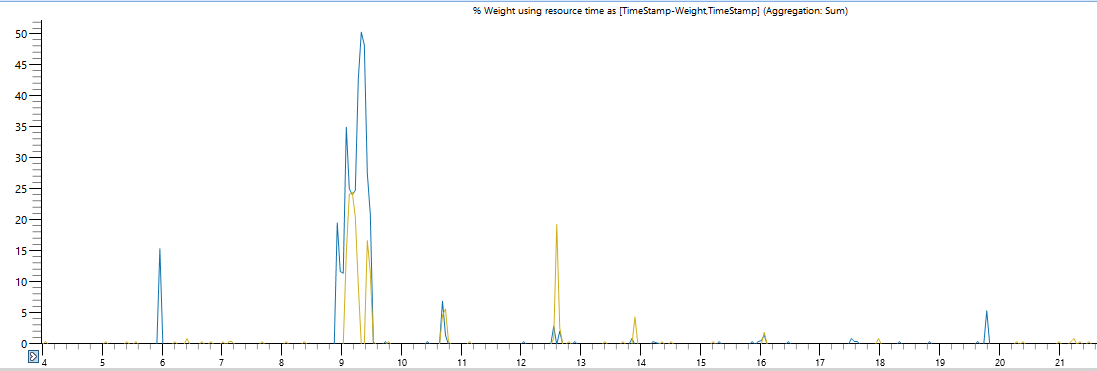
\includegraphics[width=\textwidth]{textgraph.PNG}
	\end{center}
\end{figure}
\subsection{Gtk Client}
\subsubsection{Static Analysis}
As the completion of the static analysis of the Gtk client progresses the complexity that is derived from adding a user interface on top of the original client codebase begins to reveal itself. User interfaces framework, such as Gtk, often have a single 'User Interface' object from which all other objects such as a Button or a Label are derived from, this adds a layer of inheritance complexity from the beginning of the codebase, user interface code such as event handlers can also prove to be logically complex, this ups the clyclomatic complexity of the program. User interface components also often make use of other interface objects to build up 'windows', this can cause a class to be more tightly coupled than other, simpler solutions, all of these factors intersect with each other during the development of user interface code and this shows in the results from the analysis tool. The Gtk client is less maintainable, more logically complex, has deeper layers of inheritance and tighter coupling than the text client counterpart.
\begin{table}[H]
	\centering
	\caption{Gtk Client Static Analysis Results}
	\label{my-label}
	\begin{tabularx}{\textwidth}{|X|X|X|X|X|X|}
		\hline
		\textbf{Application} & \textbf{Maintainable Index} & \textbf{Cyclomatic Complexity} & \textbf{Depth of Inheritance} & \textbf{Class Coupling} & \textbf{Lines Of Code} \\ \hline
		GtkClient & 75 &     209      &      8     &     93      &      578     \\ \hline
	\end{tabularx}
\end{table}
\subsubsection{Dynamic Analysis}
When performing dynamic analysis of the Gtk Client the process followed to capture the results was the same as that of the command line client, log in to a running server, execute commands on it which follow normal user actions and log the results. The server, in blue below, reacts similarly to requests received from the client, requests to the the server are agnostic of the client which is sending them due to the seperation of the codebases. With regards to the CPU usage required to run the client, in purple in the graph below, the highest peak of CPU usage, the login in stage where all information is gathered from the server for the initial display, has a similar cost to that of the text client. However, the latter requests, exhibit a slightly higher average cost than that of the text clients by around 5\% of CPU usage, this suggests that there is a higher cost to the returning of results received from the server than in the text client context. This would mean that there is an overlying computational buffer which is required to run the Gtk Framework on top of the communications layer implemented to access the JominiEngine server.
\begin{figure}[H]
	\caption{CPU \% usage over time, Server in blue, Client in purple.}
	\begin{center}
		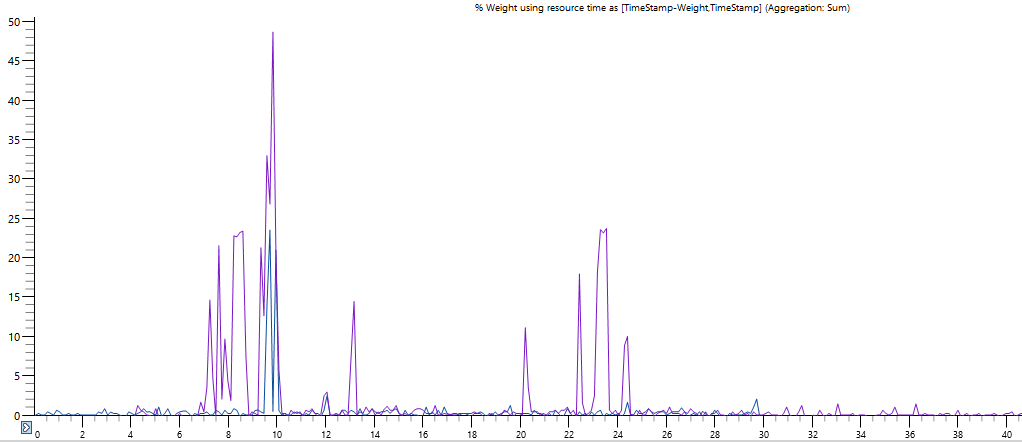
\includegraphics[width=\textwidth]{gtkclientgraph.PNG}
	\end{center}
\end{figure}
\subsection{Android Client}
\subsubsection{Static Analysis}
The static analysis of the Android client shows similar trends to the Gtk client's results, an increase in the difficulty of maintainability, a increase in complexity, deeper inheritance and tighter coupling with regards to the results of the text client. In comparison to the Gtk client however, it is less complex and has inheritance which is not as deep, this could be do to with the optimisations of the Android operating system, code which runs on a mobile device needs to be more efficient and less bloated with regards to memory usage as it runs on a device with limited resources, the inheritance depth being shallower could be a solution to that. Gtk also has to cope with running on multiple operating systems, the expenses of achieving this could mean that code which uses the framework is more bloated than code which runs only on, for example, Android or Windows.
\begin{table}[H]
	\centering
	\caption{Android Client Static Analysis Results}
	\label{my-label}
	\begin{tabularx}{\textwidth}{|X|X|X|X|X|X|}
		\hline
		\textbf{Application} & \textbf{Maintainable Index} & \textbf{Cyclomatic Complexity} & \textbf{Depth of Inheritance} & \textbf{Class Coupling} & \textbf{Lines Of Code} \\ \hline
		Android Client & 75 &  116         &   6        &    77       &     365      \\ \hline
	\end{tabularx}
\end{table}
\subsubsection{Dynamic Analysis}
When performing Dynamic Analysis of the Android client it is important to note that it is very difficult to monitor the traffic of the Android client exactly due to the fact the code runs in an emulator. The Android emulator contains all of the processes running within the phone's operating system and conceals them from the host machine, this is problematic, as when the simulator is run it is difficult to determine if the current process is a operating system task on the simulator or a spike cause by an interaction with the client. Due to this obfuscation it is difficult to determine exactly what the cause of computational weight spikes are, however, the weight spikes in this graph are much larger than those of the text client. This could be due to the fact that there are operating systems features being run at the same time which make processing less efficient and more demanding, or it could be due to the fact the Android client is less efficient, it is hard to give a truly honest answer with the tools at hand. It is possible to use the Xamarin Profiler application in order to gain a deeper insight into the current status of a Xamarin application, however this is only possible with the premium 'Visual Studio Enterprise' version of Visual Studio, which is paywalled and not accessible with a student Visual Studio license.
\begin{figure}[H]
	\caption{CPU \% usage over time, Server in brown, Android virtual machine in purple.}
	\begin{center}
		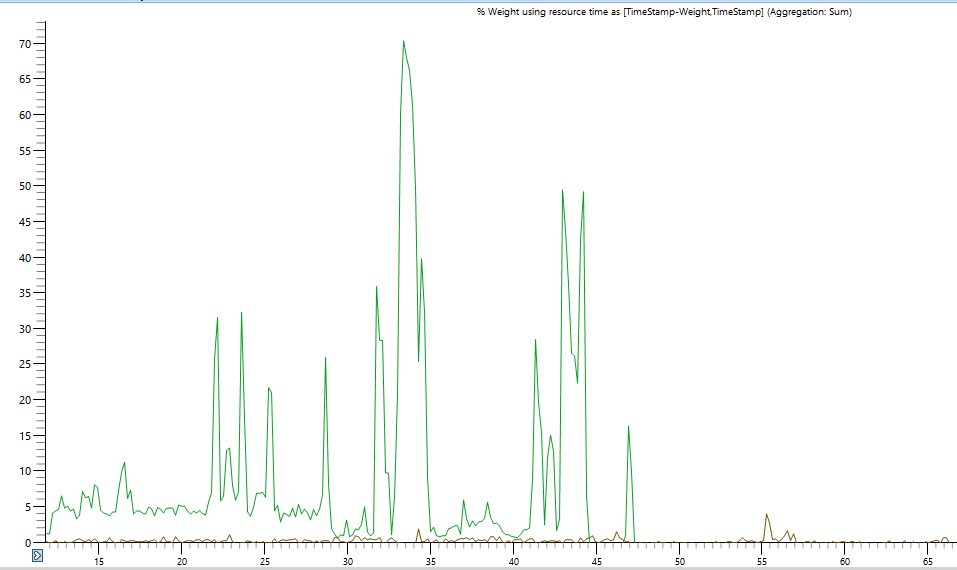
\includegraphics[width=\textwidth]{androidgraph.PNG}
	\end{center}
\end{figure}
\newpage
\section{User Evaluation}
\subsection{Methodology}
The methodology for the conducting of the user evaluation required them to carry out an test plan (Appendix Item 2) which spanned the entirety of the three sections of JominiEngine’s capability, Fief Management, Army Management, and Family Management. Due to the limited implementation of the Android client the test focused on the results of the text and graphical user interface clients only. The subjects were asked to carry out a simple task, namely, to hire troops in the fief they currently reside in, navigate to another fief not currently owned by them, and start a siege. This task encapsulates all of the potential elements of JominiEngine, recruitment for armies and the beginning of a siege, the hiring of troops who are idle recruits inside a fief owned by the player using the player’s currency, and the potential of death incurring from a siege which could possibly cause the player to have to play as their descendent if one exists. Upon the completion of the test they are presented with the SUS form which helps them to complete an evaluation of their experience with the program. The majority of the testers were members of the general public who did not work in or have large amounts of experience with using technology, most of them did not have an interest in video games. From the results of these forms the information can be extracted, then analysed and then from this analysis derive meaning from them, potentially looking for trends or signs that one client is preferred more than another. The evaluation is carried out solely on one standard computer which has enough processing power to run the graphical client with ease. This is problematic due to fact a low powered computer may suffer trade-offs with regards to memory and CPU consumption that impede usability more than on a machine that is capable of running it without issues. The result therefore will be mostly speculative, it is impossible to gain truly accurate results with regards to the usability of the clients without expanding the tests further.
\subsection{Results}
The first question of the SUS form considers how likely a user feels they are to use the system frequently. In the context of the comparison between two clients this is for the purposes of playing the game, which system could they, as players of JominiEngine, see themselves using. The results show a clear preference, the majority of those surveyed neither agree or disagree that they could see themselves using the GUI client, but show that those surveyed mostly disagree that they could see themselves frequently using the Text Client. No user showed a strongly agree preference for either client, this could suggest that there is a disenfranchisement with the mechanics of the game or that they do not find either client usable enough to play frequently with. \\
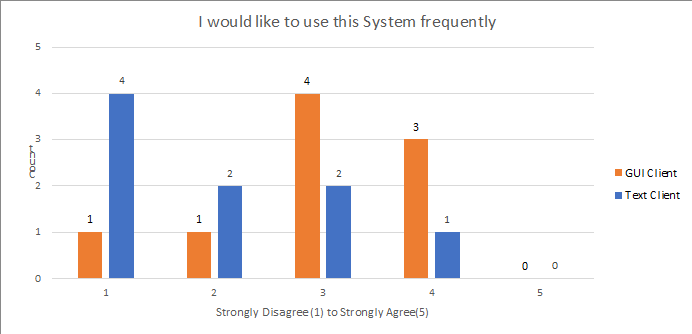
\includegraphics[width=\textwidth]{graph1.PNG}
The second question considers the complexity of the user experience, "to what extent does the user agree that the system is unnecessarily complex". This question acknowledges there may be some complexity in carrying out any operation required but asks does the user find that this goes beyond the needed level of complexity to complete the task. There is a clear result, users find the Text Client much more complex than the GUI Client, with over half of those tested picking that they mostly disagree that the GUI client is unnecessarily complex and the rest strongly agreeing with the statement. The results for the Text client are more mixed, some find the command line interface too complex to operate, impeding their progress through the test script, there is a clear choice from the tester base that the GUI client is more usable.\\
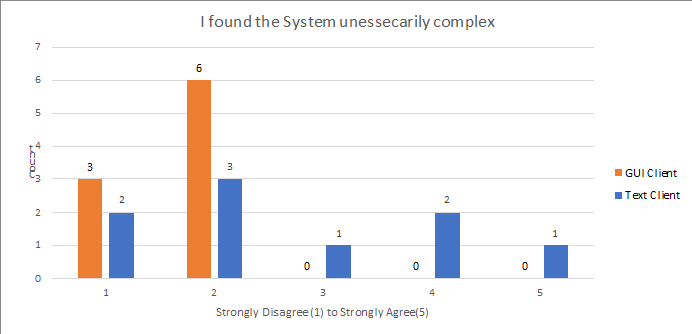
\includegraphics[width=\textwidth]{graph2.PNG}
The next question in the form asks about the ease of use of the system, this is a simple question asking the user to describe their experience completing the test steps. Both clients were reported by the users as being easy to use overall, however there was a slight preference shown for the GUI client. While most users either strongly agreed or mostly agreed with the statement there were 2 command line client users who strongly disagreed that the system was easy to use, due to the experience base of our testers this could possibly come from users who have little to no experience with using command line shells and felt alienated by the environment. The results show that adding a simple user interface on top of the client provides a gain in usability.\\
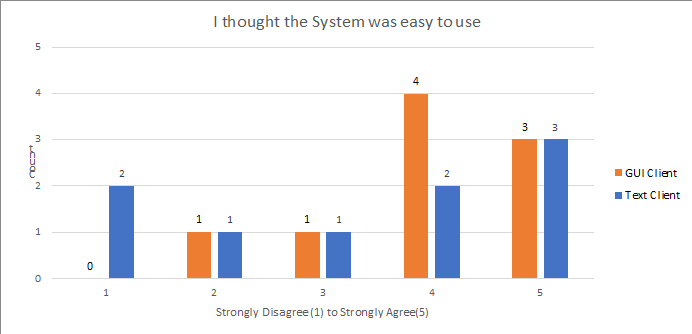
\includegraphics[width=\textwidth]{graph3.PNG}
The next question in the SUS form considers to what degree a user feels that they need technical support to make use of the system. The users during the test are provided with technical support to some extent, they are navigated through using the client via a test plan and if any issues occur they can be helped to overcome them, therefore this may be interpreted by the tester as a summation of their experience during the test. Most users thought they would need technical support to use the text client, this could arise from their inexperience with command line clients in general or it could be a function of the implementation of the interface. However, users reported that the GUI client was much easier to use, with nearly half of the users surveyed suggesting that the strongly disagree that they would need the support of a technical person to make use of the system, this suggests not only is the GUI client more usable, but it is also easier to learn to use.
\\
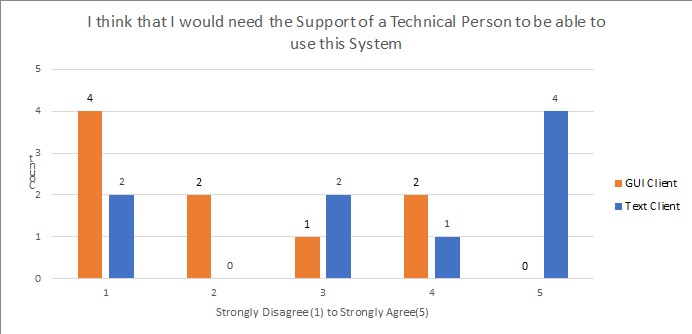
\includegraphics[width=\textwidth]{graph4.PNG}
The next two questions focus on the integration of the user interface elements, how they work and look together in harmony. The first considers whether the functions of the system are "well integrated", meaning that as components every element of the user interface works with the others, there is no part of the system that feels awkward or markedly different from another. Most users thought both clients were well integrated, favouring the GUI client slightly, this suggests that while the read-evaluate-print loop worked well to navigate the user through the test plan the comfort of a GUI to work with made for a more comfortable user experience, with the interface feeling more polished.
\\
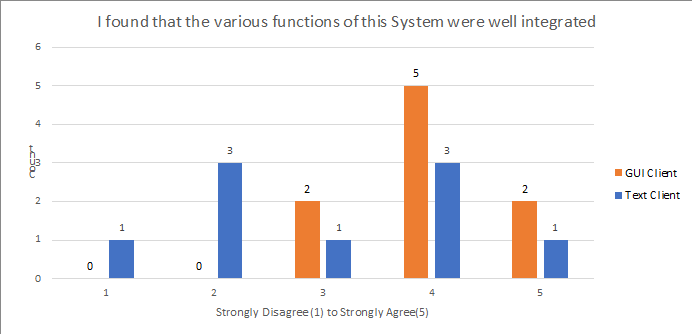
\includegraphics[width=\textwidth]{graph5.PNG}
A similar supplementary question is then asked with regards to the user interface and whether the user felt there was too much inconsistency within the system. Users strongly disagreed for both clients that there was too much inconsistency, this suggests that users felt that every element of the system's interface and user experience was coherent and nothing felt out of place throughout all the operations completed.
\\
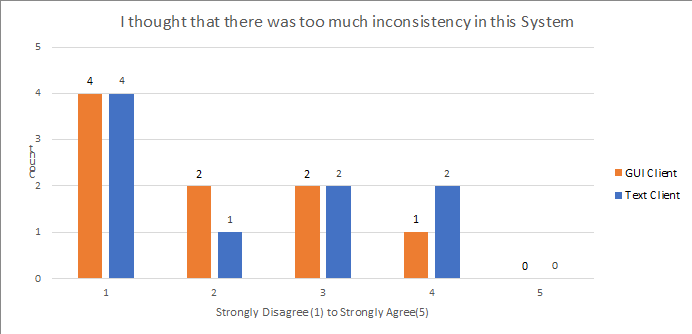
\includegraphics[width=\textwidth]{graph6.PNG}
The users are then asked to pass judgement on whether they think that other users would be able to quickly learn how to use the system. Since most of the testers came from a non technical background it involves a person who has little experience with computers passing judgement on someone else of their ability's potential to understand the system. This result showed a clear choice, every user who used the GUI client either strongly or mostly agreed that a person could work out how to use the system quickly, whereas nearly half thought that a typical user would struggle to get to grips with a command line client quickly. This suggest that adding a graphical user interface on top of the client leads to a better user experience, which users feel more comfortable in and find more intuitive.
\\
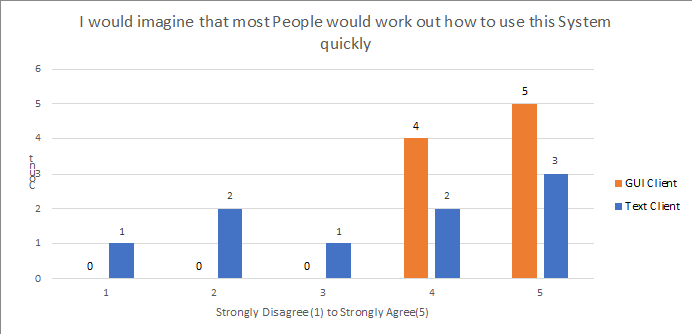
\includegraphics[width=\textwidth]{graph7.PNG}
The user is then asked whether they personal found the system cumbersome to use, do they feel that the client is working against them and impeding their progress through the test plan. The users reported once again that the graphical user interface led to a client which was much less cumbersome to use than the text client, with two thirds of users mostly disagreeing that the graphical user interface was cumbersome to use. However three users agreed to some varying degree of certainty that the text client was cumbersome to use, suggesting that users find the method of input via a read evaluate print loop is overly laborious
\\
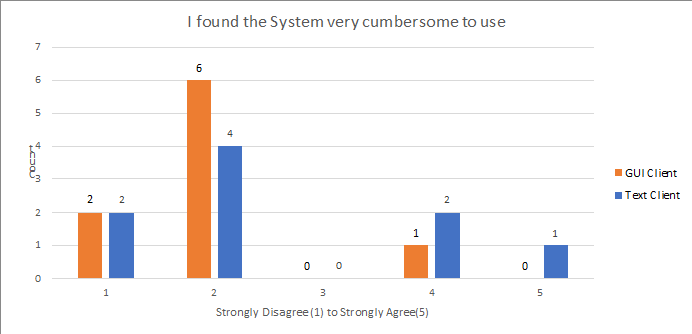
\includegraphics[width=\textwidth]{graph8.PNG}
The user then is asked to personally rate their confidence with the system overall, this could be seen as the closest question in the SUS form to an overall usability rating. While many users, over half, felt uncomfortable or indifferent using the text client to some degree, possibly for the reasons outlined before such as the need of a technical person to carry them through the plan or with regards to complexity of the interface. The graphical client fared better, with two thirds of testers surveyed feeling mostly confident with using the system, the graphical user interface removes a layer of uncertainty for most users, helping them carry out the actions they wish to, easier. 
\\
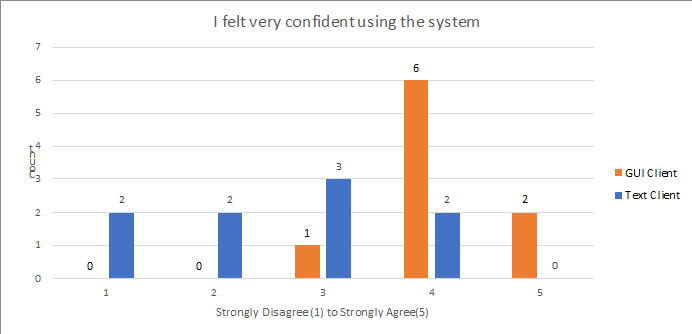
\includegraphics[width=\textwidth]{graph9.PNG}
The last question in the SUS form involves asking whether the knowledge barrier for entry into using the clients was high. Users felt that the text client required a lot of learning before the test plan could be completed, with almost half strongly agreeing that they needed to learn a lot of things before they could get going. This could be a product of the command line interface and the inexperience of the users with interfaces in this format, not only were they learning the client but they were also learning how to operate a command line at once. The graphical user interface proved to be much more successful, with all but one users surveyed disagreeing strongly or mostly that they felt they had to learn a lot of things before they could get going and complete the test plan. This could be due to the fact the graphical client came second in the testing process, they may have already acclimatised to the game via the text client and learnt more about its functions, or it could be that the interface provided a solid guide for new users of JominiEngine with which to play the game from.
\\
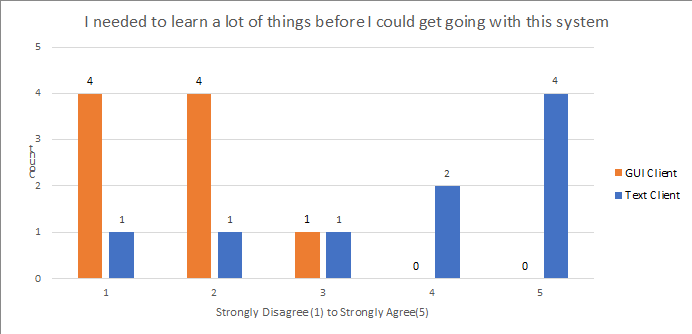
\includegraphics[width=\textwidth]{graph10.PNG}
\newpage
\section{Conclusion}
\subsection{Project Summary}
To conclude, the completion of the clients has been taken as far as it is possible to do so without large restructuring of the server codebase. The text client and its underlying codebase provide a sound structure with which to produce more clients, written in C\#, in a similar manner in the future. The Gtk client provided an usable interface to this underlying structure, allowing for a user who does not have experience with command line tools an opportunity to use the JominiEngine in future. The Android client, for all its difficulties with implementation, showed that it would be possible to create a mobile client with restructure of the server code and the codebase of the other clients that have gone before.

Modularity and extensibility were placed at the heart of the project’s aims, in order to expand the player base of JominiEngine clients which match users desires are needed to allow them choice over how they experience the game. The creation of tools in the form of build scripts allowed for developers in future to easily make use of the framework for communication with the server built upon in the clients. The abstraction of the client communications layer to a DLL, and a Portable Class Library means that future developers have a library which they can plug into any C\# codebase on any platform and communicate with the server via a robust set of fundamentals contained within the libraries. The maintainability of these respective elements of the codebase, as marked out in the static analysis stage of the technical evaluation for all clients gives JominiEngine a strong base for future developers to improve the project from.

Usability was another important component for the project which was set out at the beginning as one of the main areas for possible improvement. While a command line client was an important component of getting the project in a suitable state, allowing for testing to be performed on the communications layer to ensure it was working correctly. This was then ported to the client with a graphical user interface, speeding up the development process. The usability study conducted reported across the board preference for the graphical user interface client over the text client in terms of usability. Through increasing the accessibility of the client for users of a non technical background such as those surveyed in the usability study the possibility of JominiEngine reaching its educational goals are improved. Users are not intimidated or impeded by a client that they find easy to use and do not require large degrees of technical support to learn how to operate, this increases the immersion within the game world.

The mobile client development process was fraught with issues, however from the efforts in this space a lot has been learned about the limitations of JominiEngine and what must change fundamentally about the server before it can be ported to new platforms. The main problem with regards to extensibility is the Lidgren communications library and the limitations this places on the choice of language, which must be written in C\# in order to use the library on the client side. This limitation means that a whole host of platforms, such as native Android code or a web based client running on Node.js, are unviable solutions while this limitation remains in place. Further limitations occur with regards to the server’s usage of data structures and how these structures are imported, effectively a client has to remain tightly coupled to the server, using the same data structures in the same Visual Studio Project in order to communicate with the server. These data structures which relate to the ProtoBuf communications protocol need to be abstracted out from the server and held as a stand alone library which is then imported to any program which needs to communicate with either the client or the server. While this limitation impeded the progress of the development it does give a solid platform from which the lessons learned from the usability of graphical user interfaces in the context of JominiEngine can be applied to a future mobile client after these issues are resolved.

The evaluation process provided both technical and social insight into the success and efficacy of the clients. Through technical analysis, both static and dynamic, insight was gained into the construct of the codebase and how this affects the execution of the program in reality. Technical analysis allowed for the study to compare the effects of, for example, adding a user interface and the costs that come with that in comparison to a client which has no graphical user interface. The usability study allowed for the study to quantify the gains made from a usability standpoint and place them in perspective to the technical tradeoff. While the technical study showed little major effect with regards to complexity of the code or CPU computation time while running the program the usability study displayed major advantages from implementation of a graphical user interface.

From this study a lot has been learned about JominiEngine in its current state, where its strengths and limitations lie and how this affects creating clients for communication with the server. From the work carried out to achieve the initial goals of the study a critical analysis of the fruits of the effort has been produced, this provides information about not only JominiEngine now but provides future developers with a solid information and tooling base from which to build from in future. This helps meet the goals of the study, an extensible, portable, easy to use and computationally cheap client base for aiding users through the learning environment.

\subsection{Project Management}
With regards to the outlined expected schedule in the first deliverable there were considerable adjustments to the progress achieved in comparison to the plan outlined. This occurred both positively and negatively with regards to estimation of time constraints, while some sections, namely the development of the text based and Android clients took longer than expected, the graphical client did not take as long as estimated to complete. Original estimations expected that the command line client would take around a month to complete, however it in fact took longer. Acclimatisation to the nuances of the protocol, understanding the large codebase that was inherited from earlier projects due to the fact the server and client were deeply interlinked and tightly coupled took longer than expected, and therefore delayed the delivery of the text client. However, because of the considered approach to implementation and the importance stressed upon modularity and extensibility a codebase which was designed around portability was produced. This portability proved useful when creating a client which had a graphical user interface, the communications layer and player operation abstractions were able to be ported to the Gtk client in a shorter time than expected. Gtk, as opposed to Unity, provided a layer on top of the original client code instead of a brand new project with its own, exclusive and bespoke internal workings, speeding up the development process and making up for time lost through the slow command line implementation. The development of the Android client was fraught with issues with regards to the attempt to implement an original client natively in Java, due to issues with incompatibility in the communications layer the project had to move to using Xamarin instead, this took extra development time and slowed down the development process. After the switch to Xamarin problems regarding the portability of dynamic link libraries implemented earlier to a mobile platform and the limitations that came with that regarding to compatibility with Xamarin’s implementation of Mono slowed down the implementation further. A portable class library had to be created, this required learning about the constructs of the platform and the limitations that it comes with, slowing down development. Then more issues regarding the serialisation library, Protobuf, and the manner with which it recognises data structures it can deserialise meant that the only solution is to refactor the entire server codebase and the clients that have gone before. The Android client was therefore implemented to the full extent possible, with a communications layer that works and can send information to the server which cannot be deserialized due to the incompatibilities in data structures not being shared by both client and server, therefore a valid response cannot be returned. The writing of the textual part of the thesis and the usability testing, while performed later in the project than expected, both matched the expectations of the length of time they would take to carry out. During the initial project planning some time was left spare in case of potential problems arising, using this time and the savings from the GUI client’s development process it was possible to finish in time.

\subsection{Concerns}

\subsubsection{Legal}

As outlined in the first deliverable, the main issues with regards to legality were in the licensing of the tooling which was used and the licensing of JominiEngine itself. All tools used through the project had the correct license to use them, validated with the software vendor, or were open source and the license that they are published under was respected. With regards to the libraries used during the development, every library has had its license respected and given ample credit to the creators during the development and report process. JominiEngine itself is licensed under the MIT license, meaning that any use is allowed as long as there is accreditation for the initial author, the codebase for the clients is also published under this license, keeping the project open and extensible in the spirit of its creator. 

\subsubsection{Ethical}

Heriot Watt’s ethics framework was abided by entirely, the submitted ethics form before deliverable one was respected in full, including the full extent of the Data Protection Act clauses, mitigating any chance of subject identification. The effects of the test and the structure of the test that was carried out was clearly explained to the subjects beforehand, and they were informed that they could quit at any time during the study or up to seven days afterwards if they wished to do so. The British Computer Society's Code of Good Practice which lays out that a researcher should always aim to be ethical in their research, and should not take part in research which may be construed as to being harmful to society at large or individual citizens was also complied with in full. 

\subsubsection{Social}

Social issues concerned mostly the ability for a player to be abusive towards another; the JominEngine implemented controls for admin accounts to remove players from game, if abusive behaviour occurred and in the controlled usability study setting if such behaviour did occur the subject would be removed from the study. The usability studies were all carried out in an individual environment as opposed to a multiplayer setting, therefore a player could not interact with another during game player, because of this the concern was removed entirely. 

\subsection{Future Work}
The areas for expansion of the project mostly come from a refactoring of the server technology, to push JominiEngine onto new platforms it must abandon the tooling that has caused issues during development. The removal of Lidgren and the implementation of another communications library which fits the standardised UDP protocol would be extremely useful when exporting JominiEngine clients onto new platforms. The problems that arose in the attempted implementation of a Java based android client caused a major restructuring of the solution, however, this would not have been a necessary decision to make if the server did not use Lidgren, this would be the same for any hypothetical client written in a language other than C\#, a functional client in a language like Haskell would be impossible due to the fact there is not a Lidgren implementation it can use, this limits the availability and success of JominiEngine. 
More work is also needed to de-couple the client and server code, at the moment they are far too closely linked and it is very hard to draw a line where one ends and the other begins when looking through the codebase. The Protobuf data structures used within the server’s communications layer need to be moved to an external Portable Class Library source, they can then be imported in as a dependency, this removes any possible incompatibility issues between mobile clients and desktop clients by making them all share the same data structures for communications.
Other advancements would include the construction of new clients running on different platforms, perhaps a web application could be written which allows the user to connect from their browser. An application written using up to date JavaScript technology such as node.js could completely cut out the native code dependency entirely, all the user would need to operate JominiEngine would be a modern web browser on the device of their choosing.	
	\newpage
	\section{Bibliography}
	\printbibliography
	\newpage
	\section{Appendix}
	\subsection{Consent Form}	
	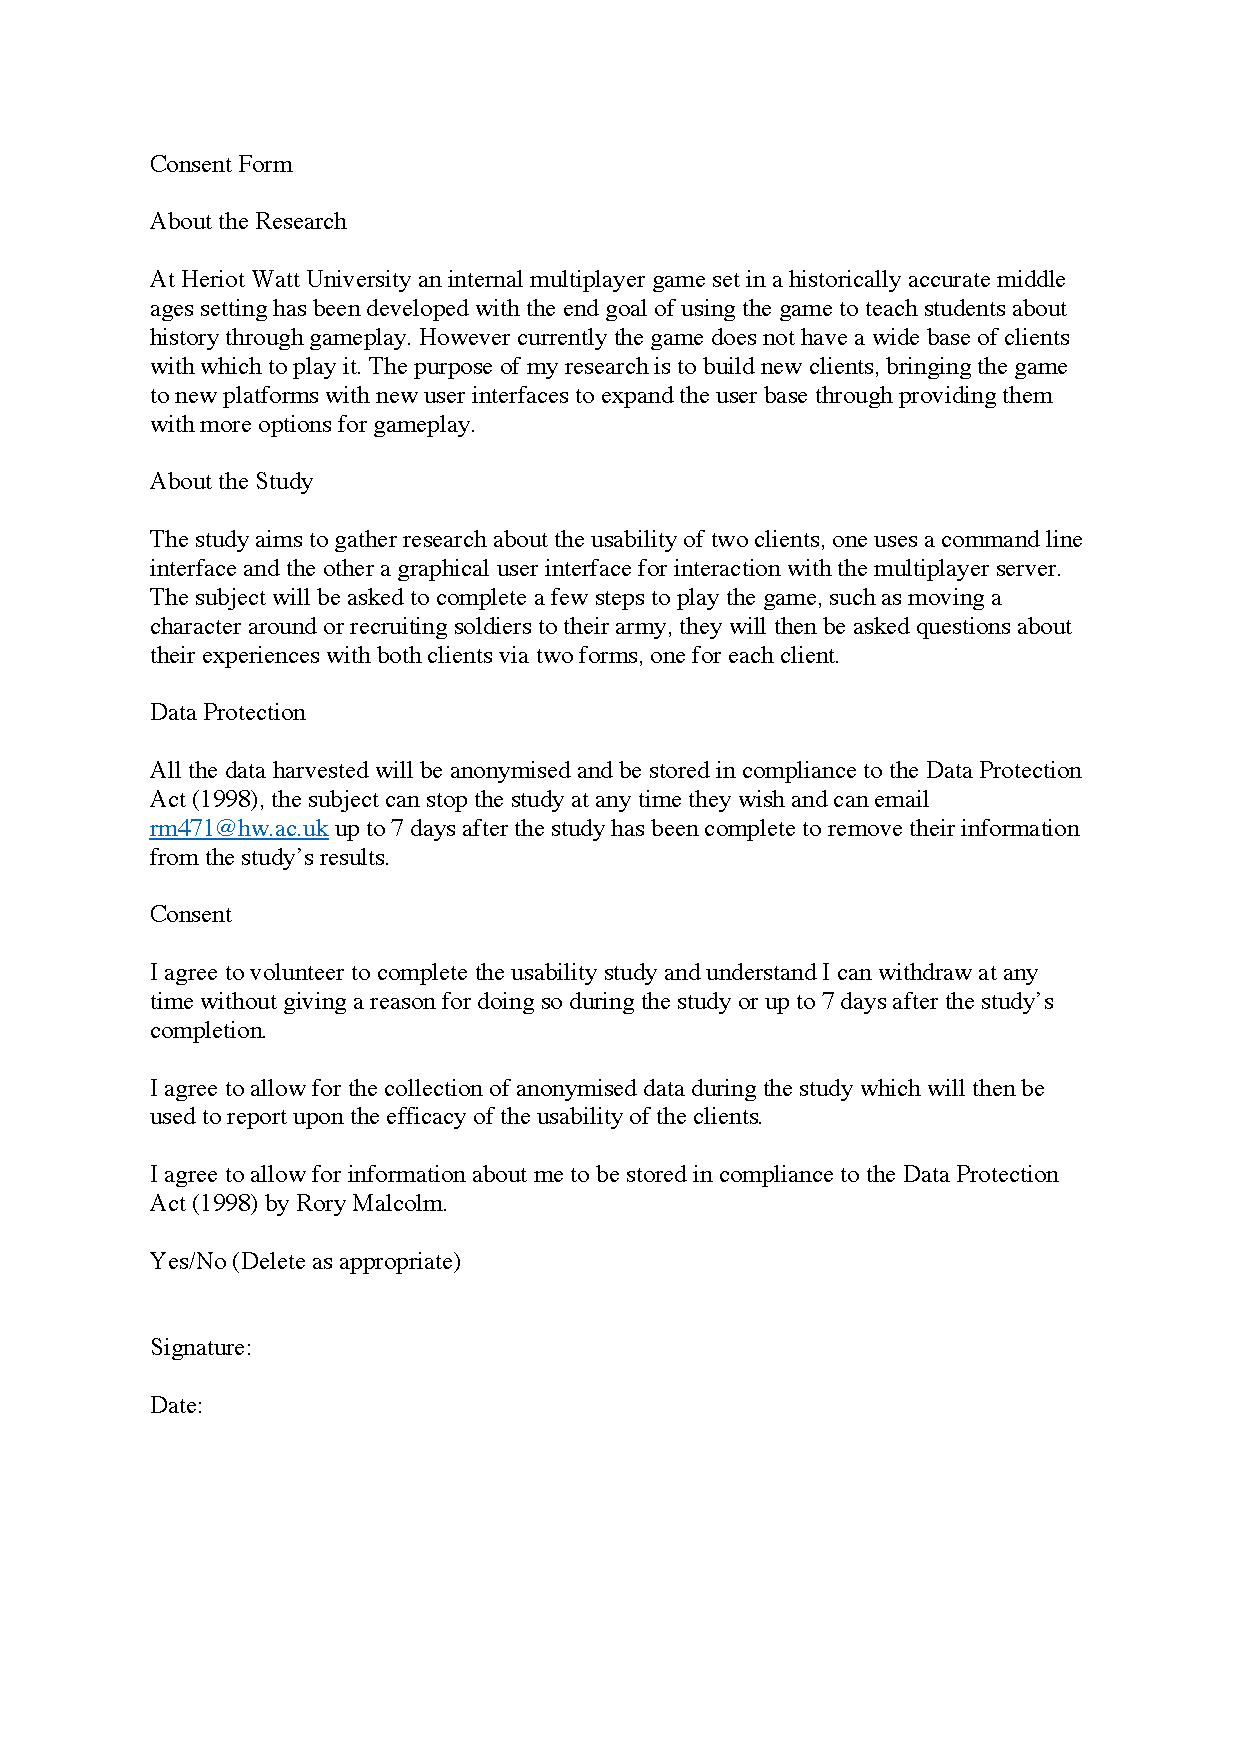
\includegraphics{consentform.pdf} 
	\subsection{Test Plan}
	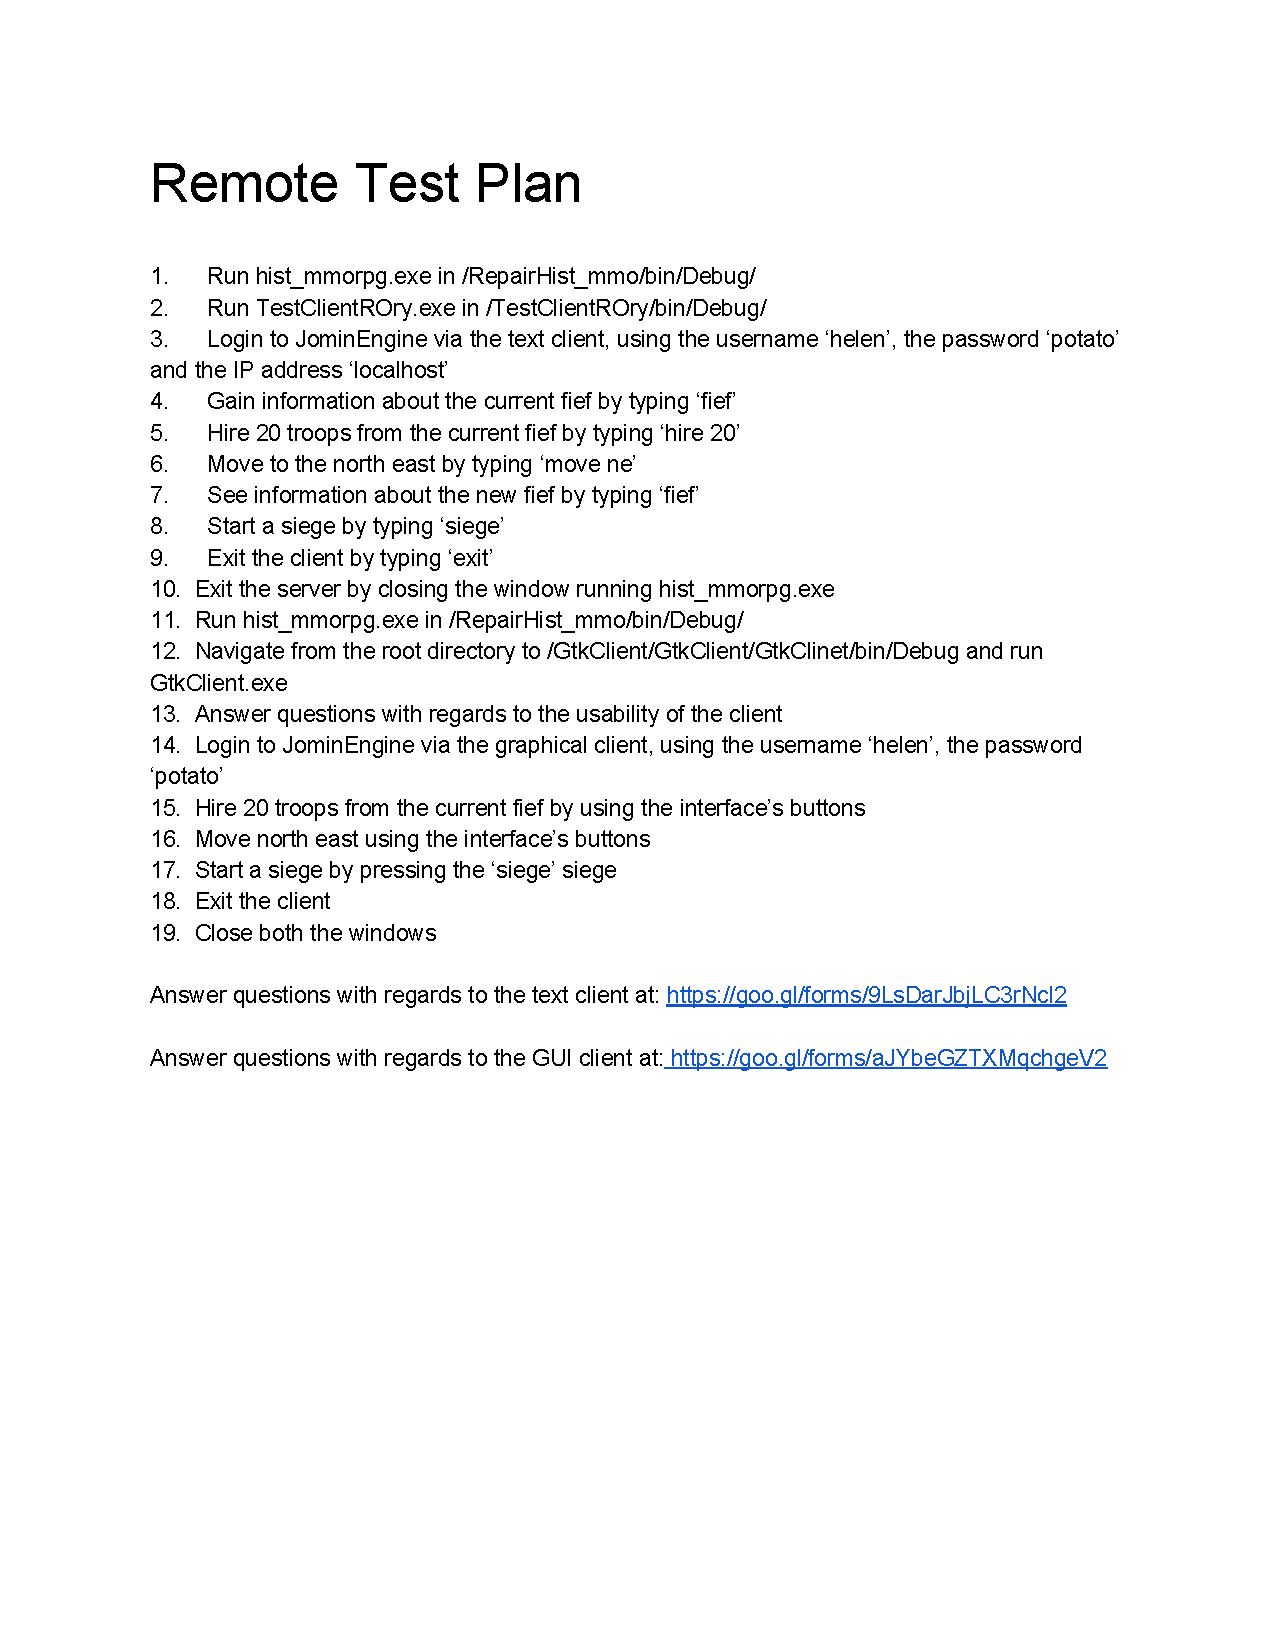
\includegraphics{RemoteTestPlanNonTechnical.pdf} 
	\subsection{SUS Form}
	\centering
	\includegraphics[page=6]{sus.pdf} 
	\subsection{UML Diagram}From David Bond's thesis\cite{DavidBond}
	\centering
	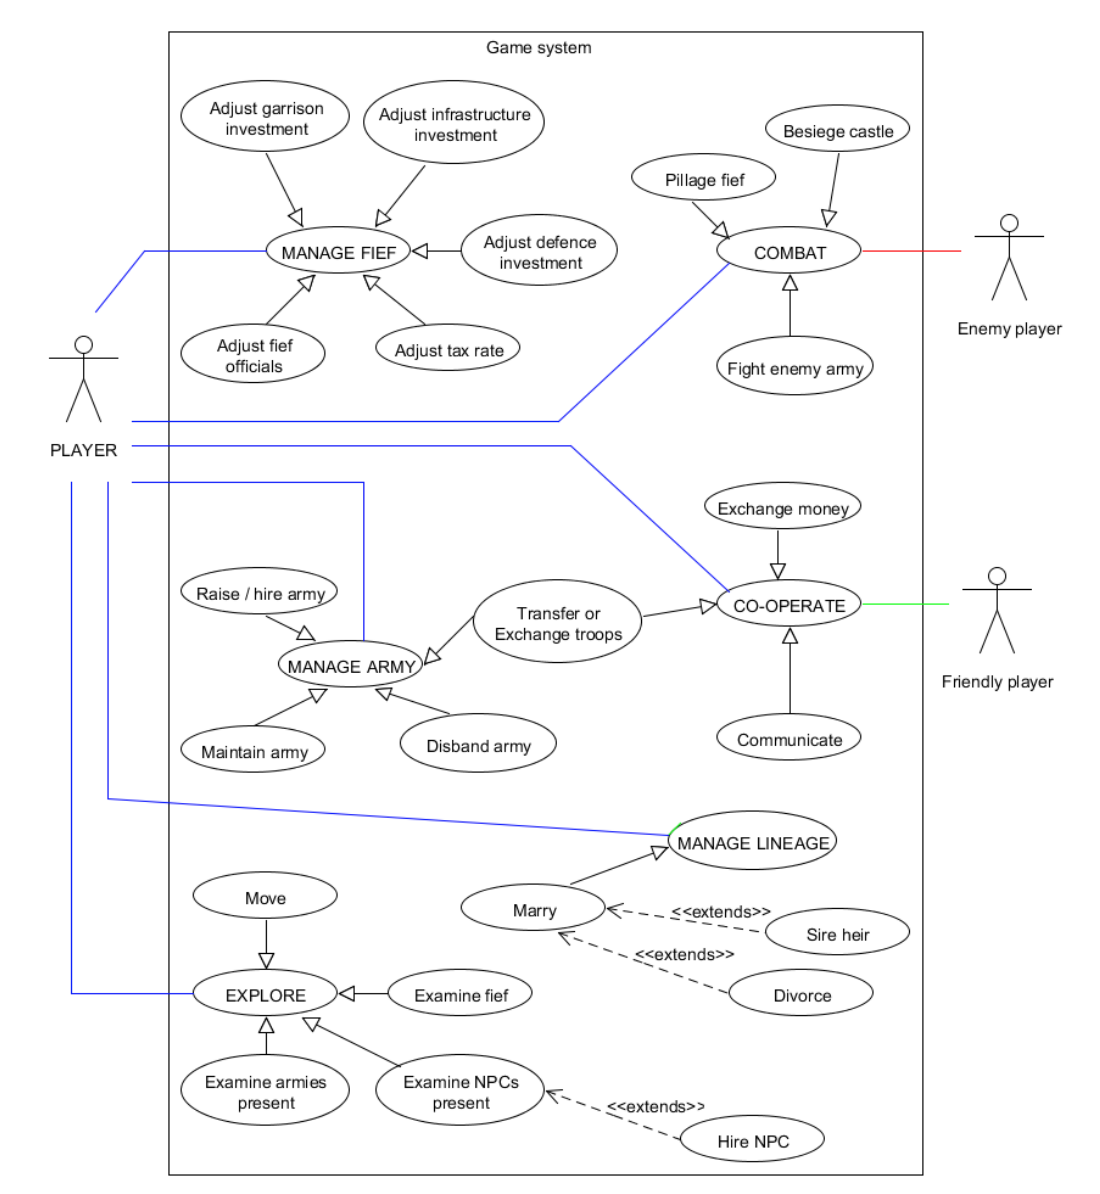
\includegraphics[width=\textwidth]{gameUML}
\end{document}
